%*****************************************						
% gi004@hdm-stuttgart.de														
%******************************************
%
% Masterdatei für die einzelnen Kapitel
%********************************************
% Allgemeine Einstellungen
%********************************************
\documentclass[
               	a4paper, 
                oneside, 
                fontsize=12pt,
                toc=bibliography]
                {report}
\usepackage[utf8]{inputenc}
\usepackage[ngerman]{babel}
\usepackage[autostyle,german=quotes]{csquotes}
\usepackage{setspace} % Package für Zeilenabstand

\onehalfspacing       %% 1,5-zeiliger Zeilenabstand
\parindent 0pt

\usepackage[
			left=30mm,
			right=30mm,
			top=30mm,
			bottom=30mm]{geometry}  % Einstellungen für die Seitenränder (links, rechts, oben, unten)

% This is a preliminary title for your thesis.
\newcommand{\thesisTitle}{it:movES - BFMC 2024}

% The time frame in which you want to write the thesis.
\newcommand{\timeFrame}{WS2023 - SS2024}

% The primary supervisor. You probably do not need to change this.
\newcommand{\supervisor}{Prof. Dr.-Ing. Reiner Marchthaler}

% The name(s) of your advisor(s). This is probably the PhD student or PostDoc that you are working with.
\newcommand{\advisor}{Zweitbetreuer: Thomas Maier}

% Select if this is a Bachelor or Master Thesis.
\newcommand{\thesisType}{Forschungsprojekt}


\usepackage[all]{nowidow}

\clubpenalty = 10000
\widowpenalty = 10000
\displaywidowpenalty = 10000

%******************************************************************************	
% Ebenen Einstellungen
%1.section, 2.subsection, 3.subsubsection, 4.paragraph, 5.subparagraph
%******************************************************************************
\setcounter{secnumdepth}{4} % Anzahl der Ebenen für Überschriften einstellen
\setcounter{tocdepth}{3} % Anzahl der Ebenen für Überschriften im Inhaltsverzeichnis einstellen


%*******************************************************************************
% Grafiken
%******************************************************************************
\geometry{verbose}
\usepackage{graphicx}
\usepackage{float} 				% Zum Ausrichten von Tabellen und Grafiken
\usepackage[export]{adjustbox}
\usepackage{listings}
\usepackage{framed,color,verbatim}
\definecolor{shadecolor}{rgb}{.9, .9, .9}

\newenvironment{code}%
   {\snugshade\verbatim}%
   {\endverbatim\endsnugshade}

%****************************************************************************
% Tabellen
%****************************************************************************
\usepackage{tabularx}	% Ermöglicht Tabellen mit Autoumbruch
\usepackage[table]{xcolor}

\setlength{\tabcolsep}{10pt}
\renewcommand{\arraystretch}{1.5}
\newcolumntype{s}{>{\columncolor{gray!40}} p{2.9cm}}

\definecolor{codegreen}{rgb}{0,0.6,0}
\definecolor{codegray}{rgb}{0.5,0.5,0.5}
\definecolor{codepurple}{rgb}{0.58,0,0.82}
\definecolor{backcolour}{rgb}{0.95,0.95,0.92}

\lstdefinestyle{mystyle}{
    backgroundcolor=\color{backcolour},   
    commentstyle=\color{codegreen},
    keywordstyle=\color{magenta},
    numberstyle=\tiny\color{codegray},
    stringstyle=\color{codepurple},
    basicstyle=\ttfamily\footnotesize,
    breakatwhitespace=false,         
    breaklines=true,                 
    captionpos=b,                    
    keepspaces=true,                 
    numbers=left,                    
    numbersep=5pt,                  
    showspaces=false,                
    showstringspaces=false,
    showtabs=false,                  
    tabsize=2
}

\lstset{style=mystyle}

%%%%%%%%%%%%%%%%%%%%%%%%%%%%%%%%%%%%%%%%%%%%%%%%%%%%%%%%%%%%%%%%%%
% Helfer während der Texterstellung
%%%%%%%%%%%%%%%%%%%%%%%%%%%%%%%%%%%%%%%%%%%%%%%%%%%%%%%%%%%%%%%%%%
\usepackage{blindtext}      % Blindtext zum Testen von Textausgaben
%\usepackage[]{showkeys} % Anzeige der Referenz-/Labelnamen im Text, Dokument auf final deaktiviert Option
\usepackage{fixme}  % ermöglicht die Verwendung von FixMes
\usepackage[pagewise]{lineno} % Zeilennummern beim Korrekturlesen sinnvoll

\usepackage{todonotes}
% überschreibt die Voreinstellung "noinline" bei TODO Notes sodass diese immer Inline angezeigt werden
\makeatletter
\presetkeys{todonotes}{inline}{}
\makeatother

\newcommand{\autor}[2][]{\todo[linecolor=green,backgroundcolor=green!25,bordercolor=green, #1]{\textbf{Autor:} #2}}


%%%%%%%%%%%%%%%%%%%%%%%%%%%%%%%%%%%%%%%%%%%%%%%%%%%%%%%%%%%%%%%%%%
%Kopf- und Fußzeile mit fancyhdr
%%%%%%%%%%%%%%%%%%%%%%%%%%%%%%%%%%%%%%%%%%%%%%%%%%%%%%%%%%%%%%%%%%
\usepackage{fancyhdr}
\fancyhf{}
%% Einstellungen für Kopf- und Fußzeile
\fancyhead[L]{\nouppercase{\leftmark}} 
\fancyfoot[C]{\thepage}

%%Linien für Kopf und Fußzeile sowie die Breite
\renewcommand{\headrulewidth}{0pt}
\usepackage[clearempty]{titlesec} % Leerseiten ohne Kopfzeile und ohne Nummerierung!

\titleformat{\chapter}[block]{\normalfont\huge\bfseries}{\thechapter}{10pt}{\huge}
\titlespacing{\chapter}{0pt}{0pt}{20pt}


%%%%%%%%%%%%%%%%%%%%%%%%%%%%%%%%%%%%%%%%%%%%%%%%%%%%%%%%%%%%%%%%%%
%Literaturverzeichnis
%%%%%%%%%%%%%%%%%%%%%%%%%%%%%%%%%%%%%%%%%%%%%%%%%%%%%%%%%%%%%%%%%%
% \usepackage[
% 	style=authortitle-ibid, 	%Zitierstil
% 	bibstyle=numeric, 		%Biblografiestil
% 	backend=biber,
% 	sortlocale=de_DE,
% 	bibencoding=utf8,
% 	hyperref,
% 	defernumbers=true,
% 	ibidtracker=context, 	% damit ebd. funktioniert
% 	isbn=false, 			% ISBN im Literaturverzeichnis
% 	url=true, 				% Url im Literaturverzeichnis
% 	doi=false]{biblatex} 

% % Lädt Anpassungen für den Zitierstil/Biblografiestil
% % Hier sind Anpassungen des Zitierstil authortitle-ibid,  und des Biblografiestil numeric an die Verwendung von Fu�noten f�r Zitate.


% , als Trenner statt ; wenn Multicite z. B. footcites angewendet wird
%\renewcommand*{\multicitedelim}{\addcomma\space}
    
%Eigener Zitierstil     
% Author: Title (Year), [Nr.], S.X     
%\makeatletter
\renewbibmacro*{cite:title}{%
  %\cbx@tempa
  %\printtext[bibhyperref]%
      \iffieldundef{year}
        {}%
         {\printtext\space\mkbibparens{\printfield{year}}%
      		}%
      		\printtext{\addcomma\space}%
          \printtext[bibhyperref]{% Falls der Title auch verlinkt werden soll hier auskommentieren
          	\mkbibbrackets{\printfield{labelnumber}}%
          } %
          } %
%\makeatother       

% Doppelpunkt zwischen Author und Titel in der Fu�note
\renewcommand*{\nametitledelim}{\addcolon\space}

% Doppelpunkt zwischen Author und Titel im Literaturverzeichnis
\renewcommand*{\labelnamepunct}{\addcolon\space}

% Titel im Literaturverzeichnis nicht mehr kursiv darstellen
\DeclareFieldFormat{title}{#1\isdot}
\DeclareFieldFormat{citetitle}{#1\isdot}

\DeclareFieldFormat[article]{title}{#1\isdot}
\DeclareFieldFormat[article]{citetitle}{#1\isdot}
\DeclareFieldFormat{journaltitle}{#1\isdot}

\DeclareFieldFormat[thesis]{title}{#1\midsentence} 
\DeclareFieldFormat[thesis]{citetitle}{#1\midsentence}

% Literaturverzeichnis Anpassung

\DeclareBibliographyDriver{thesis}{%
  \usebibmacro{bibindex}%
  \usebibmacro{begentry}%
  \usebibmacro{author}%
  \setunit{\labelnamepunct}\newblock
  \usebibmacro{title}%
  \newunit
  \printlist{language}%
  \newunit\newblock
  \usebibmacro{byauthor}%
  \newunit\newblock
  \printfield{note}%
  \newunit\newblock
  \printfield{type}%
  \newunit
  \usebibmacro{publisher+location+date}%
  \newunit\newblock
  \usebibmacro{chapter+pages}%
  \newunit
  \printfield{pagetotal}%
  \newunit\newblock
  \iftoggle{bbx:isbn}
    {\printfield{isbn}}
    {}%
  \newunit\newblock
  \usebibmacro{doi+eprint+url}%
  \newunit\newblock
  \usebibmacro{addendum+pubstate}%
  \setunit{\bibpagerefpunct}\newblock
  \usebibmacro{pageref}%
  \usebibmacro{finentry}}

\DeclareBibliographyDriver{article}{%
  \usebibmacro{bibindex}%
  \usebibmacro{begentry}%
  \usebibmacro{author/translator+others}%
  \setunit{\labelnamepunct}\newblock
  \usebibmacro{title}%
  \newunit
  \printlist{language}%
  \newunit\newblock
  \usebibmacro{byauthor}%
  \newunit\newblock
  \usebibmacro{bytranslator+others}%
  \newunit\newblock
  \printfield{version}%
  \newunit\newblock
  \usebibmacro{in:}%
  \usebibmacro{journal+issuetitle}%
  \newunit
  \usebibmacro{byeditor+others}%
  \newunit
  \usebibmacro{note+pages}%
  \newunit\newblock
  \usebibmacro{publisher+location+date}% Zusatz um Verlag und Jahr anzugeben
  \newunit\newblock
  \iftoggle{bbx:isbn}
    {\printfield{issn}}
    {}%
  \newunit\newblock
  \usebibmacro{doi+eprint+url}%
  \newunit\newblock
  \usebibmacro{addendum+pubstate}%
  \setunit{\bibpagerefpunct}\newblock
  \usebibmacro{pageref}%
  \usebibmacro{finentry}}

\renewbibmacro*{journal+issuetitle}{%
  \usebibmacro{journal}%
  \setunit*{\addspace}%
  \iffieldundef{series}
    {}
    {\newunit
     \printfield{series}%
     \setunit{\addspace}}%
  %\printtext{Vol.\addspace}%
  \usebibmacro{volume+number+eid}%
   %\printtext{Nr.\addspace}%
   \printfield{issue}%
  %\setunit{\addspace}%
  \printtext{\addspace}%
  %\mkbibparens{\usebibmacro{date}}%
  %\usebibmacro{issue+date}%
  \setunit{\addcolon\space}%
  \usebibmacro{issue}%
  \newunit}

\DeclareBibliographyDriver{misc}{%
  \usebibmacro{bibindex}%
  \usebibmacro{begentry}%
  \usebibmacro{author/editor+others/translator+others}%
  \setunit{\labelnamepunct}\newblock
  \usebibmacro{title}%
  \newunit
  \printlist{language}%
  \newunit\newblock
  \usebibmacro{byauthor}%
  \newunit\newblock
  \usebibmacro{byeditor+others}%
  \newunit\newblock
  \printfield{howpublished}%
  \newunit\newblock
  \printfield{type}%
  \newunit
  \printfield{version}%
  \newunit
  %\printfield{note}%
  \newunit\newblock
  \usebibmacro{organization+location+date}%
    \newunit
  \printfield{note}%
  \newunit\newblock
  \usebibmacro{doi+eprint+url}%
  \newunit\newblock
  \usebibmacro{addendum+pubstate}%
  \setunit{\bibpagerefpunct}\newblock
  \usebibmacro{pageref}%
  \usebibmacro{finentry}}

\renewbibmacro*{organization+location+date}{
  \iffieldundef{year}
  {}%
  {
  \printtext{(}%
  \printfield{year}%
  \printtext{)}%
  }
  }
    %\printlist{location}%
  %\iflistundef{organization}
  %  {\setunit*{\addcomma\space}}
  %  {\setunit*{\addcolon\space}}%
  %\printlist{organization}%
  %\setunit*{\addcomma\space}%
  %\mkbibparens{\
    %\mkbibparens{\usebibmacro{date}}%
  %\newunit}

\renewbibmacro*{publisher+location+date}{%
  \printlist{location}%
  \iflistundef{publisher}
    {\setunit*{\addcomma\space}}
    {\setunit*{\addcomma\space}}%
  \printlist{publisher}%
  \printtext{\space}%
  %\setunit*{\addcomma\space}%
  \mkbibparens{\usebibmacro{date}}%
  \newunit}
\usepackage[style=ieee]{biblatex}
\bibliography{Bibtex/Quellen}

% Aufteilung des Quellenverzeichnis in verschiedene Abschnitte. 

% \defbibheading{literatur}{\subsection*{Literaturquellen}}
% \defbibheading{pdf}{\subsection*{Elektronische Dokumente}}
% \defbibheading{online}{\subsection*{Internetquellen}}

% \addbibresource{./Bibtex/Quellen.bib}

%%%%%%%%%%%%%%%%%%%%%%%%%%%%%%%%%%%%%%%%%%%%%%%%%%%%%%%%%%%%%%%%%%
%Stichwortverzeichnis
%%%%%%%%%%%%%%%%%%%%%%%%%%%%%%%%%%%%%%%%%%%%%%%%%%%%%%%%%%%%%%%%%%%
\usepackage{idxlayout} %Damit der Abstand der Überschrift genauso hoch wie bei den Sonstigen Überschriften
\usepackage{makeidx}
\makeindex


% Verlinkung im Dokument 
%%%%%%%%%%%%%%%%%%%%%%%%%%%%%%%%%%%%%%%%%%%%%%%%%%%%%%%%%%%%%%%%%%
% Einstellungen für das erstellte PDF
\usepackage[
	bookmarks=true,
	bookmarksopen=true,
	bookmarksnumbered=true,
	pdftitle={it:movES
 BFMC 2024}, 
	pdfauthor={\name},
	pdfsubject={Forschungsprojekt: it:movES - BFMC 2024},
	pdfkeywords={Autonomous Driving},
	breaklinks=true,
	colorlinks=true,
	linkcolor=black,			% links in blau, black
	anchorcolor=blue,			% black
	citecolor=blue, 			% black
	filecolor=blue,				% black
	menucolor=blue,				% black
	urlcolor=blue,				% black
	pdfpagelabels=true,
	pdfstartview=Fit,
	hypertexnames=true,
	draft=false,
	plainpages=false,
	pdfpagelabels,
	hyperfootnotes=false,
	breaklinks=true]{hyperref}

\usepackage[bottom,hang,multiple]{footmisc} % Fußnoten Einstellungen
\setlength{\footnotemargin}{0pt}
\newcommand\fnsep{\textsuperscript{,}} %Komma zum manuellen trennen von Footnotes

\usepackage[all]{hypcap} % Workaaround damit Links auf Abbildungen und Tabellen auf den Beginn und nicht das Ende der Abb/Tab zeigt

% damit Urls an jedem Buchstaben umgebrochen werden, sinnvoll vor allem im Literaturverzeichnis
\usepackage[]{url}
\def\UrlBreaks{\do\a\do\b\do\c\do\d\do\e\do\f\do\g\do\h\do\i\do\j\do\k\do\l
\do\m\do\n\do\o\do\p\do\q\do\r\do\s\do\t\do\u\do\v\do\w\do\x\do\y\do\z\do\0
\do\1\do\2\do\3\do\4\do\5\do\6\do\7\do\8\do\9\do\-\do\_\do\I\do\S\do\E\do\C}%
\urlstyle{same}

%%%%%%%%%%%%%%%%%%%%%%%%%%%%%%%%%%%%%%%%%%%%%%%%%%%%%%%%%%%%%%%%%%
%Abbildgungen, Tabellen & Formeln pro Kapitel durchnummerieren 
%Tabelle 1 -> Tabelle 2.1
%%%%%%%%%%%%%%%%%%%%%%%%%%%%%%%%%%%%%%%%%%%%%%%%%%%%%%%%%%%%%%%%%%
\makeatletter
\@addtoreset{figure}{section}
\@addtoreset{table}{section}
\makeatother
\renewcommand{\thefigure}{\thesection.\arabic{figure}} % Abbildung
\renewcommand{\thetable}{\thesection.\arabic{table}}  % Tabelle
\renewcommand{\theequation}{\arabic{section}.\arabic{equation}} %Formeln


%%%%%%%%%%%%%%%%%%%%%%%%%%%%%%%%%%%%%%%%%%%%%%%%%%%%%%%%%%%%%%%%%%
%	Glossaries: Abkürzungsverzeichnis
%%%%%%%%%%%%%%%%%%%%%%%%%%%%%%%%%%%%%%%%%%%%%%%%%%%%%%%%%%%%%%%%%%
\usepackage[
   acronym, % Abkürzungsverzeichnis erstellen
   toc, % zum Inhaltsverzeichnis hinzufügen
   shortcuts]{glossaries} 

% Name des Abkürzungsverzeichnis anpassen
\addto\captionsngerman{\renewcommand\glossaryname{Glossar}}
\deftranslation[to=ngerman]{Acronyms}{Abkürzungsverzeichnis}
\deftranslation[to=ngerman]{Glossary}{Glossar}

%-----------------------------------------------------------------
% Eigener Stil für Abkürzungsverzeichnis
%-----------------------------------------------------------------
\newglossarystyle{mylist}{%
  \renewenvironment{theglossary}%
     {\begin{longtable}[l]{@{}lp{0.75\textwidth}@{}}} %Damit Tabelle Linksbündig am Rand beginnt
     {\end{longtable}}%
  \renewcommand*{\glossaryheader}{}%
  \renewcommand*{\glsgroupheading}[1]{}%
  \renewcommand*{\glossaryentryfield}[5]{%
    \glsentryitem{##1}\textbf{\glstarget{##1}{##2}} & ##3\glspostdescription\space ##5\\}%
  \renewcommand*{\glossarysubentryfield}[6]{%
     &
     \glssubentryitem{##2}%
     \glstarget{##2}{\strut}##4\glspostdescription\space ##6\\}%
%  \renewcommand*{\glsgroupskip}{ & \\}%
	 \renewcommand{\glsgroupskip}{}%
}
%-----------------------------------------------------------------
\renewcommand*{\glspostdescription}{} %Punkt am Ende jeder Beschreibung deaktivieren
\makeglossaries % Glossar erstellen

%************************************************************************************************
\begin{document}

\clubpenalty = 10000
\widowpenalty = 10000
\displaywidowpenalty = 10000

%\linenumbers 			%Zeilennummern; zum Korrekturlesen einkommentieren

%\pagestyle{empty}		% Keine Kopf-/Fusszeilen auf den ersten Seiten.

%****************************************
%Include
%****************************************
% Deckblatt
\begin{titlepage}
\begin{center}

\begin{minipage}[b]{.25\linewidth}
    \centering
    
\includegraphics[width=\linewidth]{./Pictures/HdM_Logo.jpg}
\end{minipage}

\normalsize{Fakultät Druck und Medien}\\
\large{\textbf{Studiengang Medieninformatik}}\\[0.5cm]

\LARGE{{\thesisType} Thesis}\\
\normalsize{zur Erlangung des akademischen Grades Bachelor of Science}\\[0.7cm]
\Huge{\textbf{\thesisTitle}}

%\vspace{0.5cm}

%\Large{in Zusammenarbeit mit Leomedia GmbH}

\vspace{1cm} 

\Large{\textbf{\name}} \\[3pt]  

\large{\textbf{19. Juni 2023}}

\vspace{0.3cm} 

\large{Matrikelnummer: 39307} \\
\large{Bearbeitungszeitraum: \timeFrame} \\ 

\vspace{1cm}

\large{\textbf{Betreuer}}\\
\vspace{0.2cm}
\supervisor\\
\normalsize{Hochschule der Medien}\\
\vspace{0.2cm}
\large{\advisor}\\
\normalsize{Leomedia GmbH}

%\includegraphics[width=0.13\linewidth, right]{./Pictures/Löwe.png}
%
\includegraphics[width=0.25\linewidth, right]{./Pictures/Leomedia_Logo.png}

\end{center}
\end{titlepage}
\vfill		% Deckblatt
% % Erklärung

\section*{Erklärung}

Hiermit erkläre ich, dass ich die vorliegende Arbeit selbständig angefertigt habe. Es wurden nur die in der Arbeit ausdrücklich benannten Quellen und Hilfsmittel benutzt. Wörtlich oder sinngemäß übernommenes Gedankengut habe ich (mit Ausnahme dieser Erklärung) als solches kenntlich gemacht.
\vspace{4\baselineskip}

\begin{tabular}{lp{2em}l}
 \hspace{5cm}   && \hspace{4cm} \\
 \cline{1-1}\cline{3-3}
 Ort, Datum     && Unterschrift
\end{tabular}  	% Erklärung
% Kurzfassung, Abstract
\renewcommand\abstractname{Zusammenfassung}

\begin{abstract}
\autor{Aaron J. Müller}
In dieser Arbeit wird die Weiterentwicklung des it:movES Softwarestacks für autonome Modellfahrzeuge im Kontext der Teilnahme bei der Bosch Future Mobility Challenge (BFMC) dokumentiert.
Um bei dem Wettbewerb konkurrenzfähig zu sein, sollen Schwächen des bestehenden Softwarestacks identifiziert und ausgebessert werden.

Den Schwerpunkt bilden hierbei einerseits die Implementierung eines umfassenden Behavior-Trees, und andererseits die Entwicklung eines Lateralreglers basierend auf dem Stanley-Controller.
Die Ergebnisse sollen in das auf ROS basierende Gesamtsystem integriert werden.
Ein weiterer wichtiger Teil ist die Anpassung des Stacks auf die aktualisierten Regularien, welche neue Szenarien und eine größere Karte enthalten.
Außerdem wurde die bereitgestellte Hardware angepasst.

Die umgesetzten Änderungen werden im Wettbewerb erprobt und mit Ansätzen anderer Teams verglichen, um diese sowie die Gesamtstrategie zu evaluieren.

\end{abstract}

\clearpage

 		% Abstract
\tableofcontents
\thispagestyle{empty}
% Abkürzungsverzeichnis
\newacronym{dt.}{dt.}{deutsch}
\newacronym{engl}{engl.}{englisch}
\newacronym[description={United States of America, \acs{dt.} Vereinigte Staaten von Amerika}]{USA}{USA}{United States of America}

\newacronym{Abb}{Abb.}{Abbildung}
\newacronym{Anm}{Anm.}{Anmerkung}
\newacronym{html}{HTML}{Hypertext Markup Language}
\newacronym{URL}{URL}{Uniform Resource Locator}
\newacronym{AWS}{AWS}{Amazon Web Services}
\newacronym{GCP}{GCP}{Google Cloud Platform}
\newacronym{S3}{S3}{Simple Storage Service}
\newacronym{GC}{GC}{Google Cloud}
\newacronym{GCS}{GCS}{Google Cloud Storage}
\newacronym{IAM}{IAM}{Identity and Access Management}
\newacronym{SSE}{SSE}{Server-Side Encryption}
\newacronym{SSE-S3}{SSE-S3}{Server-Side Encryption with S3 Managed Keys}
\newacronym{SSE-KMS}{SSE-KMS}{Server-Side Encryption with AWS Key Management Service}
\newacronym{SSE-C}{SSE-C}{Server-Side Encryption with Customer-Provided Keys}
\newacronym{API}{API}{Application Programming Interface}
\newacronym{SDK}{SDK}{Software Development Kit}
\newacronym{REST}{REST}{Representational State Transfer}
\newacronym{HTTP}{HTTP}{Hypertext Transfer Protocol}
\newacronym{CLI}{CLI}{Command Line Interface}
\newacronym{CRUD}{CRUD}{Create, Read, Update, Delete}
\newacronym{JSON}{JSON}{Javascript Object Notation}
\newacronym{XML}{XML}{Extensible Markup Language}
\newacronym{FUSE}{FUSE}{Filesystem in Userspace}
\newacronym{kb}{KB}{Kilobytes}
\newacronym{GB}{GB}{Gigabytes}
\newacronym{TB}{TB}{Terabytes}
\newacronym{CRR}{CRR}{Cross Region Replication}
\newacronym{SRR}{SRR}{Same Region Replication}
\newacronym{ADC}{ADC}{Application Default Credentials}	
\pagenumbering{arabic}
\setcounter{page}{3}
\glsaddall[types={\acronymtype}] % damit auch nicht benutzte Abkürzungen erscheinen
\begin{doublespacing}	% Zeilenabstand 2.0
\printglossary[type=\acronymtype,nonumberlist, nogroupskip]
\end{doublespacing}


%%%%%%%%%%%%%%%%%%%%%%%%%%%%%%%%%%%%%%%%%%%%%%%%%%%%%%%%%%%%%%%%%%
% Abbildungsverzeichnis ausgeben
%%%%%%%%%%%%%%%%%%%%%%%%%%%%%%%%%%%%%%%%%%%%%%%%%%%%%%%%%%%%%%%%%%
\clearpage
\phantomsection				
\addcontentsline{toc}{chapter}{\listfigurename}		
\listoffigures 

%%%%%%%%%%%%%%%%%%%%%%%%%%%%%%%%%%%%%%%%%%%%%%%%%%%%%%%%%%%%%%%%%%
% Tabellenverzeichnis ausgeben
%%%%%%%%%%%%%%%%%%%%%%%%%%%%%%%%%%%%%%%%%%%%%%%%%%%%%%%%%%%%%%%%%%
\phantomsection
\clearpage
\phantomsection		
\addcontentsline{toc}{chapter}{\listtablename}
\listoftables 
\clearpage

\chapter{Einleitung}

Das folgende Kapitel dient der Einführung in die Problemstellung, Motivation sowie Ziele und Vorgehensweisen der vorliegenden Arbeit.

\section{Problemstellung und Motivation}

Die steigende Menge an Binärdaten im Kontext von Web Services, die in verschiedenen Anwendungen generiert werden, stellt eine große Herausforderung dar. Dabei ist es von großer Bedeutung, dass diese Daten sicher, zuverlässig und schnell gespeichert und abgerufen werden können. Vor diesem Hintergrund stellen sich Fragen nach der Auswahl eines geeigneten Speichersystems, das die Anforderungen wie Performance, Verfügbarkeit, Sicherheit und API-Anbindung erfüllt.  Zudem müssen Mechanismen bereitgestellt werden, um den Zugriff auf die Daten zu beschränken durch sichere, zeitlich begrenzte URL’s.\\

Diese Bachelorarbeit richtet sich auf das Problem einer Full-Service-Ticketing Software „leoticket“, die vom Unternehmen Leomedia GmbH entwickelt wurde. 
Leomedia GmbH ist ein Unternehmen, das Software für Medienunternehmen wie Zeitungsverlage, Radiosender, Veranstalter, Künstler und Kulturvereine entwickelt. \textcite{leomedia-web}\\
Leoticket ist eines der vielen Produkte von Leomedia, dass Services wie Online-Kartenvorverkäufe, Abendkassen, den Einlass bei der Veranstaltung, Statistiken und Abrechnungen und die Planung der Veranstaltung realisiert.\textcite{leomedia-web}\\ 

% Kontext des Problems beschreiben

Das Problem liegt bei der Speicherung und Bereitstellung der Daten. Da es sich um Replikationen der Daten handelt, ist die Belastung des Systems hoch. Hohe Daten werden herumgeschoben. Die Bandbreite ist bei der Übertragung begrenzt. Ein weiteres Problem ist die Bereitstellung der Daten über Email Anhänge. Anhänge dürfen eine bestimmte Speichergröße nicht überschreiten. Wenn Ticketkäufer zehn oder 100 digitale Tickets kaufen, dann müssen diese über Email Anhänge bereitgestellt werden.\\


\section{Zieldefinition und Vorgehensweise}

Ziel dieser Arbeit ist die Realisierung eines Prototypen anhand der ausgewählten Speicherlösung die Binärdaten durch sichere, zeitlich begrenzte URLs bereitstellt. Dabei werden folgenden Fragen gestellt:

\begin{itemize}
	\item Welches Speichersystem ist im Hinblick auf Kosten, Performance und Verfügbarkeit für die Persistenz von Binärdaten besonders geeignet? 
	\item Wie kann man Daten durch sichere, zeitlich begrenzte URL's bereitstellen?
\end{itemize}

Im Rahmen der vorliegenden Bachelorarbeit werden verschiedene Arten von Speichersystemen untersucht, um die Forschungsfragen zu beantworten. Dabei erfolgt eine Analyse der aktuell verfügbaren Speichertechnologien auf dem Markt hinsichtlich ihrer Eigenschaften wie Sicherheit, Verfügbarkeit, Performance und Kosten. Bei der Berücksichtigung der Integration des Speichersystems in Software-Produkte wird auch die API-Anbindung des Speichersystems betrachtet. Zur sicheren Bereitstellung von Dateien werden zudem geeignete Cloud-Provider miteinander verglichen. Kosten- und Performance-Kalkulationen werden durchgeführt, um eine geeignete Speicherlösung auszuwählen. Die Ergebnisse werden anschließend ausgewertet.\\

Im Zuge der prototypischen Umsetzung werden die ausgewählten Technologien implementiert und Testdateien zur Verfügung gestellt. Nach der Durchführung von Messungen zur Performance auf Testdaten erfolgt eine Zusammenfassung der Implementierung.\\

Abschließend werden die Ergebnisse nochmals dargestellt und interpretiert sowie Schwächen und Grenzen des Prototyps aufgezeigt. Zur Einhaltung des roten Fadens der Arbeit werden die gestellten Forschungsfragen beantwortet und potenzielle Anwendungen des Prototyps aufgelistet.

 
\chapter{Projekt Überblick}

\section{Motivation}
\autor{Medjen Izairi}
In mehrmonatiger Zusammenarbeit zwischen den Bosch-Experten und Hochschulprofessoren und Studenten soll eine zuverlässige Lösung für die Kernfunktionen eines autonom fahrenden Fahrzeugs im Maßstab 1:10 entwickelt werden. Diese Kernfunktionen umfassen in einer Miniatur-Smart-City unterschiedliche Aufgaben. Dazu gehören Spurhaltung, sicheres Navigieren in Kreuzungen, adäquate Reaktionen auf Verkehrslichter, präzise Navigation basierend auf Lokalisierungsdaten und die Fähigkeit zur sicheren Interaktion mit anderen Verkehrsteilnehmern.\cite{boschfumobility}
Zu den herausfordernden Aufgaben gehört unter anderem die präzise Spurhaltung, um eine sichere und stabile Fahrweise zu gewährleisten. Ebenso wird die Fähigkeit des Fahrzeugs, sich sicher durch Kreuzungen zu navigieren, intensiv getestet und weiterentwickelt. Dabei stehen adäquate Reaktionen auf Verkehrslichter im Fokus, um eine reibungslose Interaktion mit der Umgebung zu gewährleisten. 
Des Weiteren legt das Projekt einen Schwerpunkt auf die präzise Navigation, basierend auf hochgenauen Lokalisierungsdaten. Die Entwicklung einer robusten Lokalisierungstechnologie ist entscheidend, um das Fahrzeug in der Miniatur-Smart-City präzise und zuverlässig zu positionieren. Gleichzeitig wird die Fähigkeit des Fahrzeugs zur sicheren Interaktion mit anderen Verkehrsteilnehmern, wie Fußgängern und anderen Fahrzeugen, eingehend erforscht und optimiert.

\newpage

 
\section{Zieldefinition und Vorgehensweise}
\autor{Medjen Izairi}
Die Herangehensweise an die Projektentwicklung gliedert sich in vier Hauptdomänen: Perception, Sensing, Planning und Controlling. Jede Domäne umfasst spezifische Aufgaben, die in vier Unterphasen durchgeführt werden: Vorbereitungsphase, Planungsphase, Implementierungsphase und Testphase. Die klare Struktur erstreckt sich von der Einarbeitung und Forschung über die Planung und Umsetzung bis hin zu umfassenden Tests. Zusätzlich zur Softwareentwicklung werden Hardware-Aspekte berücksichtigt, darunter Autolieferungen und die Entscheidung für zusätzliche Hardwareteile. Die Lieferung und der Einbau dieser Teile sind entscheidende Schritte, um sicherzustellen, dass die entwickelten Technologien sowohl auf der Software- als auch auf der Hardwareebene effektiv zusammenarbeiten. Das gemeinsame Ziel besteht darin, die Miniatur-Smart-City zu einem realistischen Testumfeld zu machen, in dem die entwickelten Technologien ihre Wirksamkeit unter realitätsnahen Bedingungen unter Beweis stellen können.


\newpage

\section{Aufbau der Arbeit}

\autor{Aaron Müller}

Nach dem Projektüberblick beschäftigt sich das dritte Kapitel mit dem Gesamtprojekt.
Es werden die Rahmenbedingungen der \gls{BFMC} 2024 erläutert, insbesondere Veränderungen zu vergangengen Wettbewerben. 
Außerdem wird der it:movES Softwarestack erläutert, auf dem diese Arbeit aufbaut, und es werden Hardware-Upgrades am bereitgestellten Fahrzeug diskutiert.

Die folgenden Kapitel Lateralregler und Behavior Tree befassen sich mit den großen Aufgabenfeldern, die den Kernpunkt dieser Arbeit bilden. 
Diese Kapitel sind in sich wie eine klassische Forschungsarbeit gegliedert, und können so auch unabhängig voneinander betrachtet werden.

Das letzte Kapitel schließt die Arbeit ab, in dem ein Fazit zum Gesamtprojekt gezogen wird.
Dabei werden die Ergebnisse diskutiert und Ausblicke für weitere Forschungsarbeiten im Kontext des it:movES Softwarestacks gegeben.
\chapter{Gesamtprojekt}

\section{BFMC 2023}
\autor{Felix Anslinger}
Da die \gls{BFMC} ein jährlich stattfindender Wettbewerb ist, gab es in der Vergangenheit bereits Teilnehmergruppen der Hochschule Esslingen, welche an der \gls{BFMC} teilnahmen. Zumal das Fahrzeug jedes Jahr von Bosch neu bereitgestellt wird, und nach dem Wettbewerb zurück gegeben werden muss, kann das Fahrzeug der vorherigen Teilnehmer nicht übernommen werden. 

Anders ist die Situation jedoch in Bezug auf die Software, welche auf dem Fahrzeug läuft. Es gibt diesbezüglich kein Verbot dafür, bereits existierenden Softwarestacks weiterzuentwickeln und diese als Grundlage zu verwenden. Die bei der letztjährigen \gls{BFMC} 2023 verwendete Softwarearchitektur, stellt bereits Programmcode für viele unterschiedliche Domänen eines autonomen Fahrzeugs zur Verfügung und unterteilt den Softwarestack außerdem in mehrere einzelne Komponenten. Somit folgt der Softwarestack dem \gls{SoC} Designprinzip, wodurch sich die unterschiedlichen Komponenten weitgehend unabhängig voneinander weiterentwickeln lassen (siehe Abbildung \ref{fig:softwarestack2023}). Dies ist eine maßgebende Eigenschaft des Softwarestacks und unter anderem Grund dafür, weswegen sich dieser gut als Basis für die \gls{BFMC} 2024 eignet.
\begin{figure}[H]
    \centering
    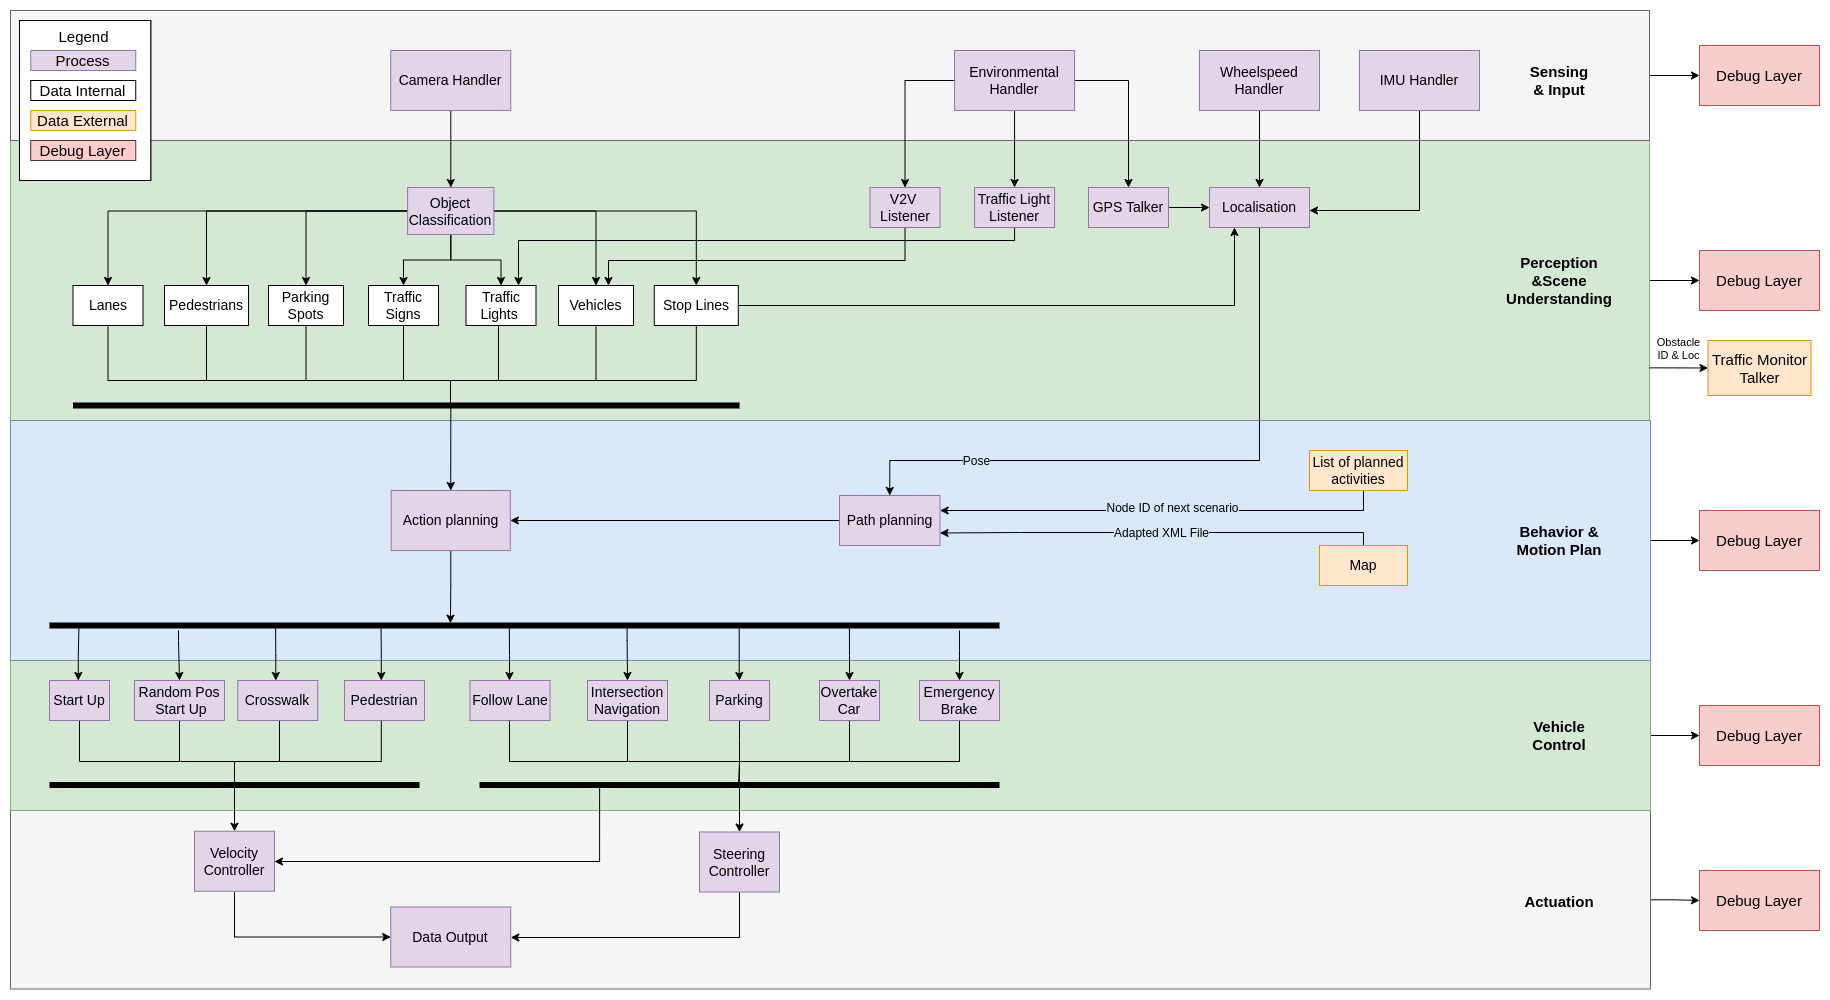
\includegraphics[width=1\linewidth]{Pictures/Project_Architecture_4_DriverlES.png}
    \caption{Softwarestack BFMC 2023}
    \cite{softwarestackBFMC2023}
    \label{fig:softwarestack2023}
\end{figure}

Die Kommunikation zwischen den einzelnen Komponenten ist durch die kollektive Implementierung von \gls{ROS} realisiert. Somit können Komponenten, wie beispielsweise die Objekterkennung, wichtige Informationen publizieren, welche dann von anderen Komponenten abgefragt und verarbeitet werden können. Durch diese Kommunikation und der Entwicklung der einzelnen Komponenten des \gls{BFMC} 2023 Softwarestacks, ist dieser bereits in der Lage, folgende Fahrsituationen zu bewältigen:
\begin{itemize}
    \item Halten der Spur
    \item Einparken
    \item Überholen von Fahrzeugen
    \item Anhalten bei Fußgängerüberwegen, Ampeln und bestimmten Verkehrsschildern
    \item Navigieren einer Kreuzung
\end{itemize}

Um diesen Softwarestack effizienter und unabhängiger von dem Fahrzeug testen zu können, wurde außerdem eine Simulationsumgebung in der Spiel-Engine Unity entwickelt (siehe Abbildung \ref{fig:unitySimulator}). Diese kann sich, anhand von \gls{ROS}, mit dem Softwarestack verbinden, wodurch simulierte Kamera-Feeds von Unity als Dateninput generiert werden können.  Die durch den Softwarestack berechneten Outputs werden dann in der Simulation umgesetzt, wodurch die Software mittels „Software in the Loop“ getestet werden kann. Dies kann im Zuge der \gls{BFMC} 2024 eingesetzt werden, um die Auswirkung von Weiterentwicklungen an dem Softwarestack in verschiedenen Fahrsituationen zu testen.

\begin{figure}[H]
    \centering
    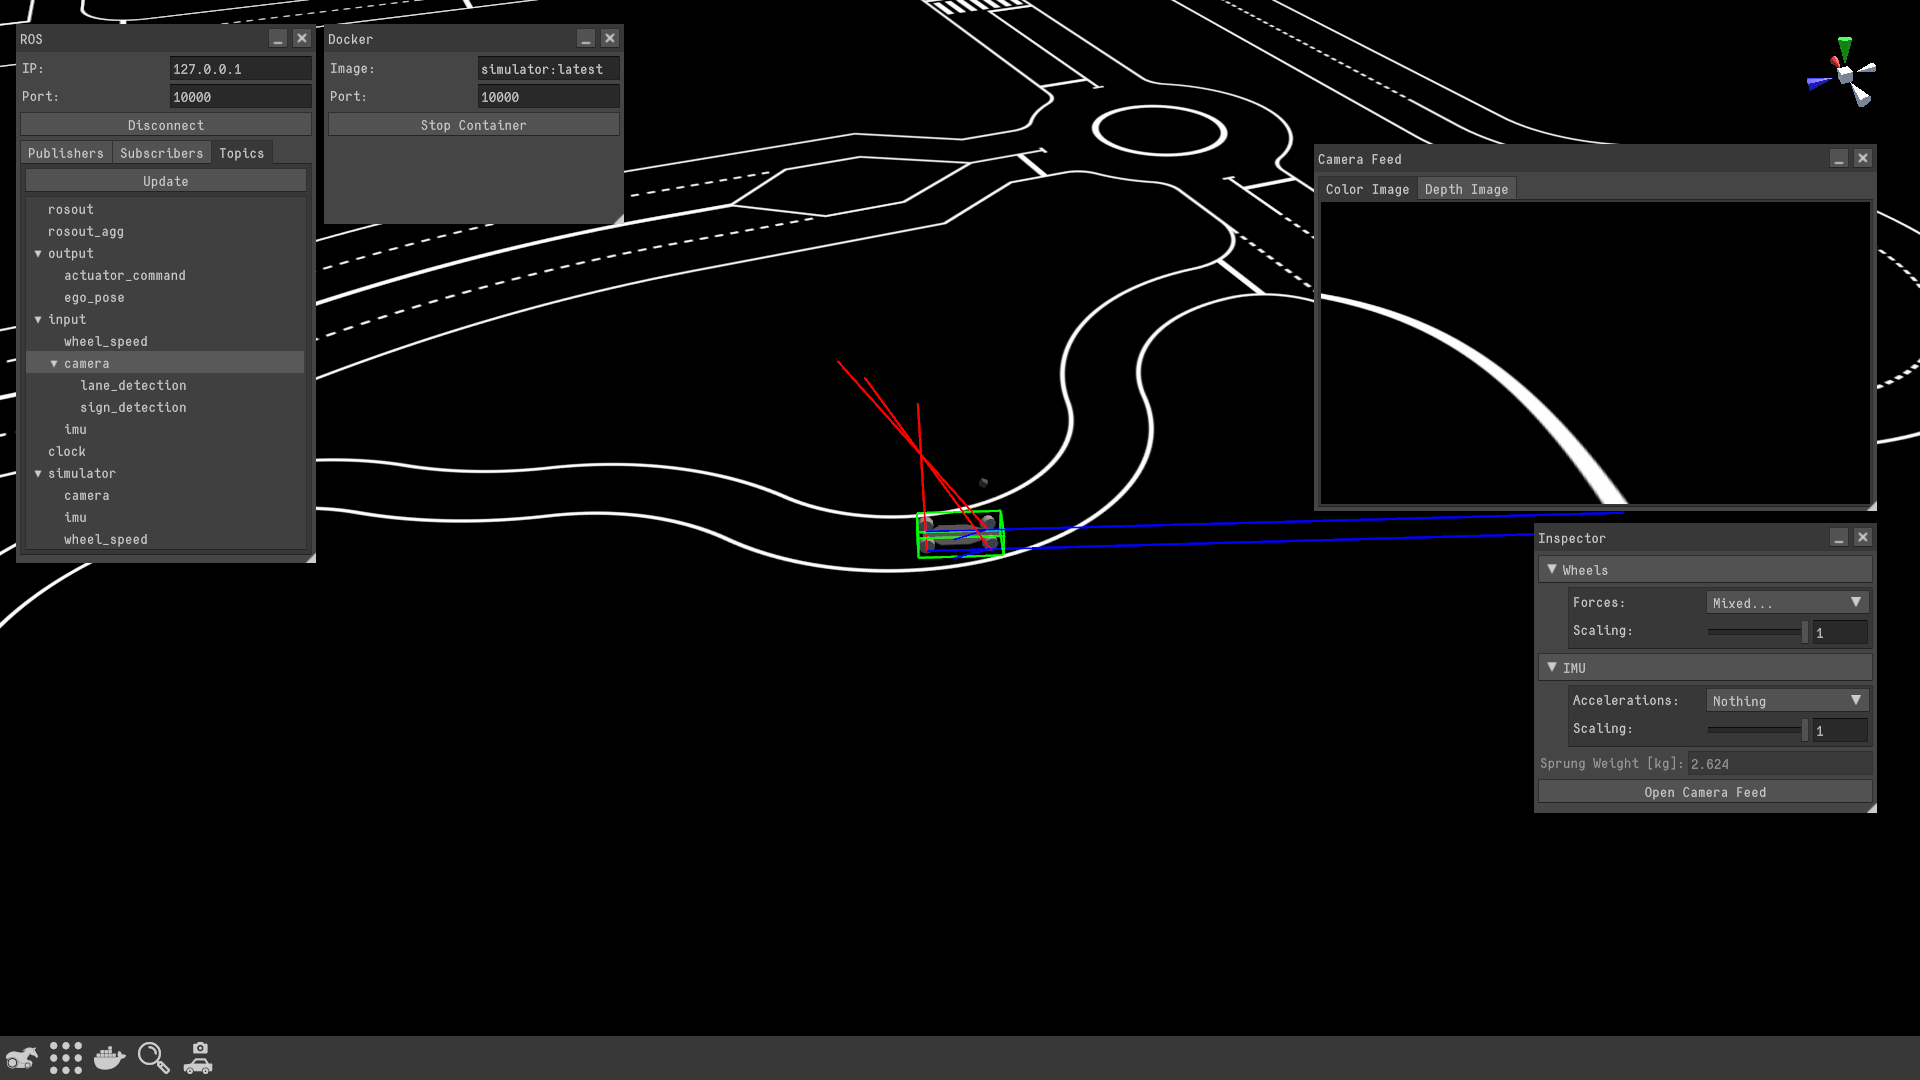
\includegraphics[width=1\linewidth]{Pictures/preview-2.png}
    \caption{Unity Simulator}
    \cite{hs_esslingen_git}
    \label{fig:unitySimulator}
\end{figure}

\newpage

\section{BFMC 2024}

\subsection{Bereitgestellte Hardware}
\autor{Felix Anslinger}

Für die \gls{BFMC} 2024 wird ein Elektro-Modellfahrzeug in dem Maßstab von 1:10 bereitgestellt. Dieses Fahrzeug besteht aus folgenden Bestandteilen: \cite{bosch_bfmc_competition_regulation}
\begin{itemize}
    \item Fahrgestell
    \item Bürstenloser Gleichstrommotor
    \item Servomotor für die Lenksteuerung
    \item \gls{IMU} für Orientierung und Geschwindigkeitsrückmeldung
    \item Mikrocontroller für Low-Level-Interaktion mit dem Fahrzeug (Nucleo F401 RE)
    \item Hauptplatine zur Entscheidungsfindung (Raspbery pi4, 8 GB)
    \item Weitwinkelkamera (Raspberry camera v3, wide)
    \item Stromverteilungsplatine zur Verwaltung der Systemleistung
    \item Batterie zur Stromversorgung
    \item Fahrzeugkarosserie zur Verdeckung der Komponenten
\end{itemize}

Diese Komponenten sind, wie in Abbildung \ref{fig:schaltplanFahrzeug} dargestellt, miteinander verbunden. 
\begin{figure}[H]
    \centering
    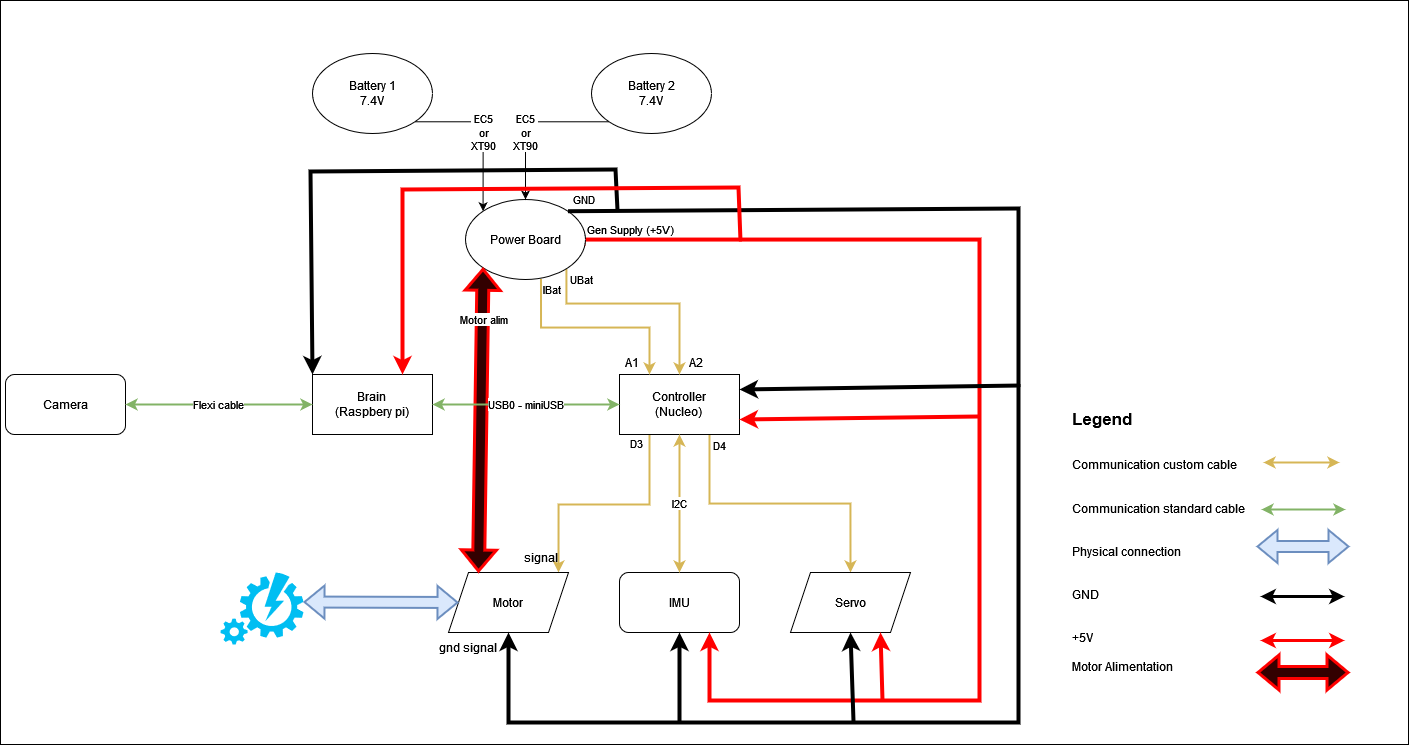
\includegraphics[width=1\linewidth]{Pictures/ConnectionDiagram.png}
    \caption{Schaltplan der Hardware des Fahrzeuges}
    \cite{bosch_bfmc_competition_documentation}
    \label{fig:schaltplanFahrzeug}
\end{figure}

\newpage
\subsection{Hardware Upgrades}
\autor{Gamze Isik, Aaron Müller}

Für die Ausstattung der Hardware wird der NVIDIA Jetson Orin NX \cite{jetson-orinNX} in Verbindung mit dem Carrierboard JETSON ORIN IO \cite{jetson-orinIO} sowie dem Reflection Sensor QTR-1A\cite{reflection-sensor} verwendet, um das Fahrzeug entsprechend zu modifizieren. Der Einsatz des NVIDIA Jetson Orin NX erweist sich als vorteilhafter im Vergleich zum Raspberry Pi mit 8GB, da der Jetson Orin NX eine höhere Leistungsfähigkeit besitzt. Dieser übernimmt die Funktion des Gehirns und führt Berechnungen durch, während \gls{ROS} ausgeführt wird. 
Die höhere Leistung ist besonders auch für KI-Algorithmen notwendig, wie z.B. einer Semantischen Segmentierung oder Objekterkennung.\\

Die Reflection Sensoren werden oft in Robotik- und Elektronikprojekten eingesetzt, um Linienverfolgungsaufgaben oder die Erkennung von Oberflächen zu ermöglichen. Im Kontext des zuvor genannten Textes wird der QTR-1A Reflectance Sensor verwendet, um die gefahrene Distanz und die Geschwindigkeit des Fahrzeugs zu messen, indem er die reflektierte Infrarotstrahlung von Markierungen auf den Rädern erfasst.\\

Auf die Anschaffung einer neuen Kamera verzichtet, stattdessen wird die mitgelieferte Raspberry Pi Kamera genutzt.
Alternativ wäre es möglich gewesen, eine Stereokamera wie z.B. die Intel Realsense\cite{intel-realsense} zu verwenden, welche zusätzlich zu den Bilddaten Tiefeninformationen liefert.
Das von den Regularien vorgeschriebene Budget reicht jedoch nicht für die zusätzliche Verwendung der teuren Kamera, sodass Abstände von Objekten auf dem Bild errechnet werden müssen.
Sollte sich die Berechnung schwieriger gestalten als gedacht, können auch günstige Ultraschall- oder LiDAR-Sensoren verwendet werden.

\newpage
\subsection{Regularien}
\autor{Gamze Isik}

Die Regularien für die \gls{BFMC} 2024 unterscheiden sich von denen des letzten Jahres. Die Rennstrecke weist eine andere Route im Vergleich zum Vorjahr auf. Die Strecke umfasst verschiedene Straßenelemente, darunter:

\begin{itemize}
    \item Gerade Streckenabschnitte
    \item Kurven
    \item Kreuzungen (mit 3 oder 4 Straßenbegegnungen)
    \item Parallelparkplätze
    \item Einspurige Straßen
    \item Zweispurige Straßen
    \item Autobahnen
    \item Kreisverkehre
    \item Einbahnstraßen
    \item Rampen
\end{itemize}

\begin{figure}[!h]
    \centering
    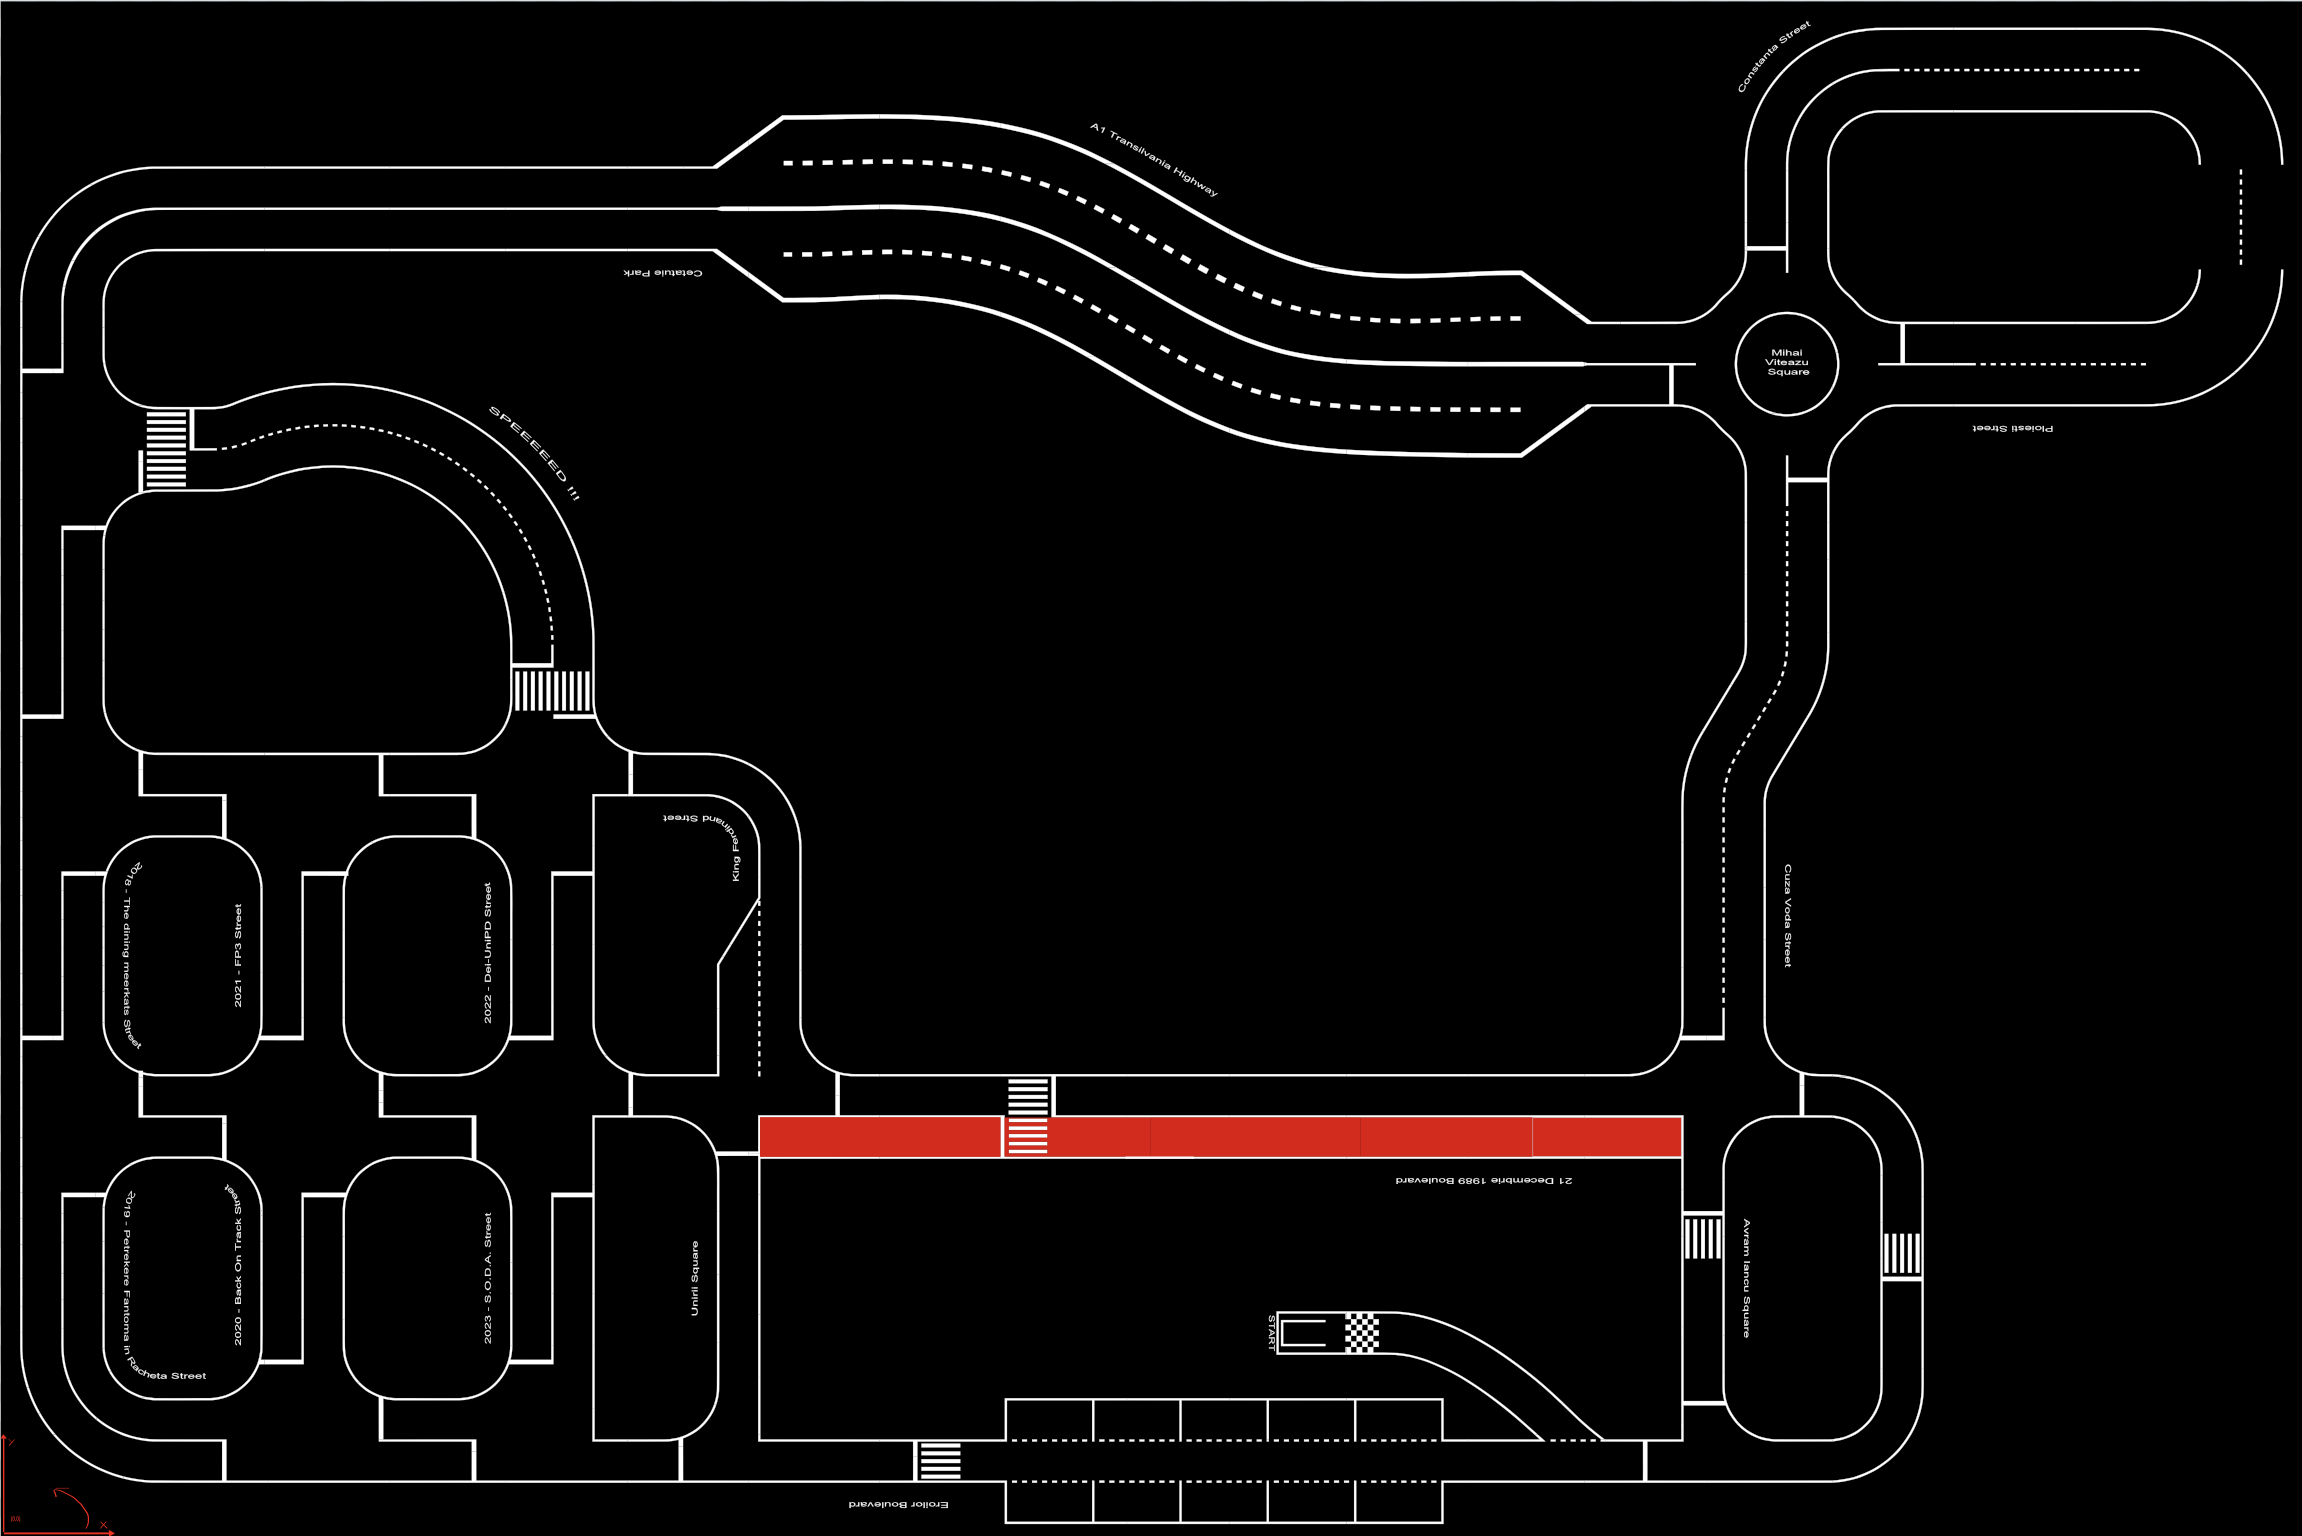
\includegraphics[width=1\linewidth]{Pictures/RaceTrack.png}
    \caption{\gls{BFMC} 2024 Race Track}
    \label{fig:race-track}
\end{figure}

\newpage

Die Fahrspurbreiten auf der rechten und linken Seite betragen jeweils etwa 35 cm, während die weißen Fahrspurlinien 2 cm breit sind (sofern nicht anders angegeben).\cite{bfmc-roadMark}

\begin{figure}[!h]
    \centering
    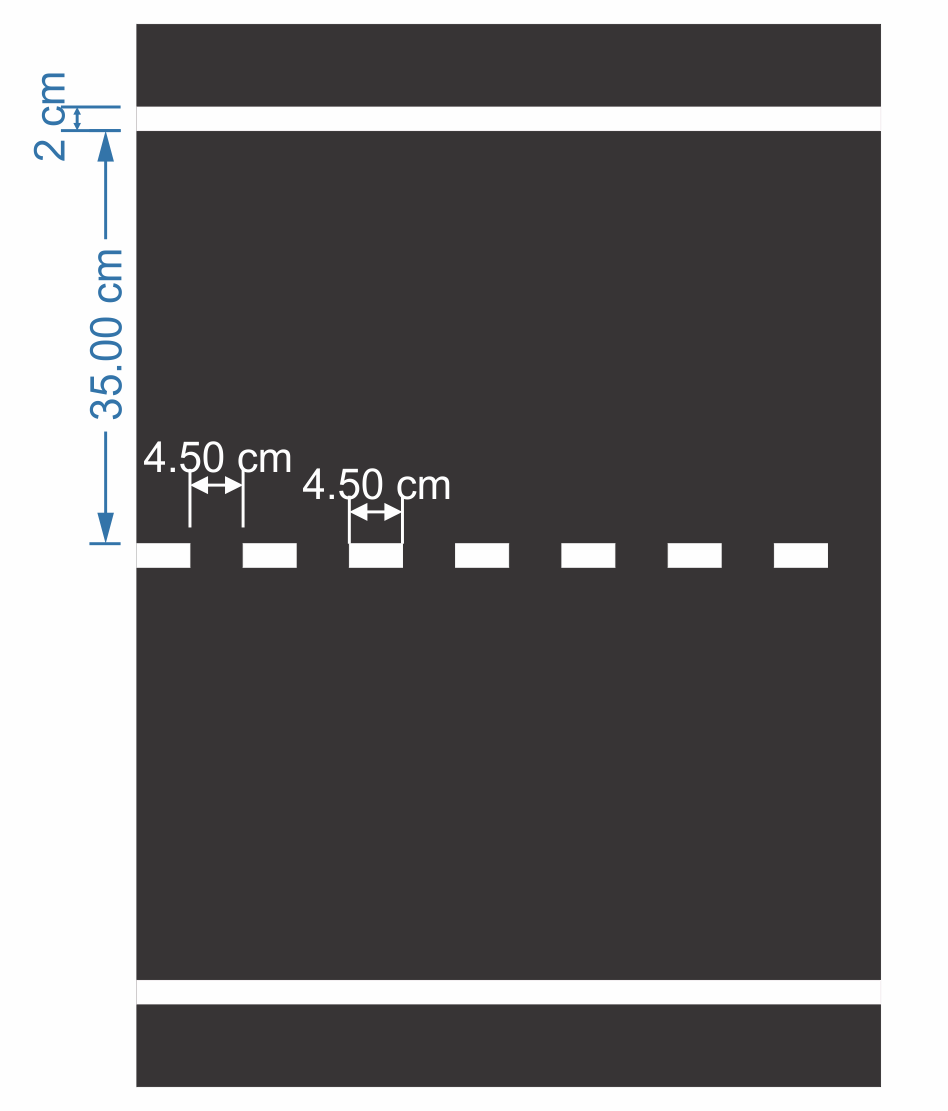
\includegraphics[width=0.5\linewidth]{Pictures/road.png}
    \caption{Straßen Bemessung}
    \cite{bfmc-roadMark}
\end{figure}

Des Weiteren werden Verkehrsregeln aufgestellt, die in der Tabelle \ref{traficRules} aufgelistet sind.\\

Die \gls{BFMC} stellt eine Reihe von Systemen bereit, die sich mit dem Aspekt der Konnektivität in der Herausforderung befassen. Diese Systeme replizieren die Umgebung einer intelligenten Stadt und bieten den Teilnehmern vielfältige Möglichkeiten zur Entwicklung ihrer Projekte. Dadurch können sie Daten fusionieren und validieren sowie geteilte Daten anfordern und senden. Die verfügbaren Systeme sind:

\begin{itemize}
    \item Ein Lokalisierungssystem
    \item Ein Echtzeit-Verkehrsüberwachungssystem
    \item Intelligente Ampeln
    \item Fahrzeugkommunikation
\end{itemize}

\textbf{Lokalisierungssystem}\\

Es handelt sich um eine physische Box, die während der Fahrt auf dem Auto platziert wird. Es bietet die ungefähre Position des Fahrzeugs auf der Strecke mit einer Frequenz von etwa 5 Hz. Das System hat einen maximalen Fehlerradius von 20 cm und eine Verzögerung von bis zu 0,5 Sekunden.\cite{bfmc-vehicle2everyth}\\
\newpage
\textbf{Verkehrskommunikationssystem}\\

Jedes Auto muss Daten an ein hauseigenes Verkehrskommunikationssystem senden, darunter die Arten von Hindernissen (basierend auf Ereignissen), Fahrzeuggeschwindigkeit, Fahrzeugposition und Fahrzeugausrichtung, einmal alle 3 Sekunden (oder weniger). Die Daten werden verwendet, um die Details der gerade durchgeführten Fahrt des Autos nachzubilden.\cite{bfmc-vehicle2everyth}\\

\textbf{Intelligente Ampel}\\

Die Ampeln teilen ihren Status im Netzwerk mit, indem sie ihren Farbzustand und ihre Position auf der Karte anzeigen. Die Frequenz der gesendeten Nachrichten beträgt 1 Hz.\cite{bfmc-vehicle2everyth}\\

\textbf{Fahrzeugkommunikation}\\

Fahrende Fahrzeuge übermitteln ihre Positionen im Netzwerk mithilfe von Rohwerten aus dem Lokalisierungssystem. Die Frequenz der gesendeten Nachrichten beträgt 5 Hz, wobei Genauigkeit und Verzögerung direkt mit dem GPS korreliert sind.\cite{bfmc-vehicle2everyth}

\subsubsection{Technische Herausforderung}\\

\quote{In der technischen Herausforderung startet das Fahrzeug des Teams von einem festgelegten Punkt (entweder der START-Position oder der zufälligen Position, die vom Jury ausgewählt wurde, wenn das Hindernis gewählt wurde).\\
Ab diesem Zeitpunkt ist nur der Einsatz eines Dashboards als Computer und laufende Software erlaubt, das als Teil des Startcodes bereitgestellt wird (die Verwendung anderer Steuerungen, Geräte oder Anwendungen ist verboten). Die App dient als Überwachungsanwendung, in der das teilnehmende Team, das Organisations- und Jury-Team oder andere Teilnehmer in Echtzeit den Zustand des Fahrzeugs überprüfen können. Jedes Team kann sein Dashboard an seine eigenen Bedürfnisse anpassen oder es von Grund auf neu erstellen. Die technische Herausforderung sollte direkt von der App aus gestartet werden. Ein Verkehrslicht mit rotem Licht wird am Startpunkt vorhanden sein. Die Jury gibt das Startsignal durch Drücken ihres eigenen Startknopfes und Ändern der Farbe des Verkehrslichts von Rot auf Grün. Das Fahrzeug muss den Start der Fahrt autonom erkennen und den spezifischen Szenarien (beschrieben im Abschnitt zur Punktevergabe) des Teams folgen.\\
Teams können ihre optionalen Szenarien für zusätzliche Punkte auswählen, solange die Laufzeit eingehalten wird (Die Fahrt selbst wird bei Erreichen des 10-Minuten-Limits gestoppt). Szenarien können in beliebiger Reihenfolge angegangen werden, aber Teams müssen die Organisatoren über die ausgewählten optionalen Herausforderungen informieren und möglicherweise den Pfad ihres Fahrzeugs mitteilen (falls der zufällige Startpunkt nicht ausgewählt wurde).} \cite{bfmc-competition}
% Entwicklung eines verbesserten Lateral-Controllers

\chapter{Lateralregler}

\section{Einleitung und Motivation}
\autor{Aaron J. Müller}
Damit ein autonomes Fahrzeug zuverlässig einer berechneten Solltrajektorie folgen kann, ist ein robuster und effizienter Regler notwendig.
Häufig wird dieser in zwei Teilprobleme aufgeteilt: Ein Longitudinalregler regelt die Fahrgeschwindigkeit, während ein Lateralregler die Lenkung des Fahrzeugs steuert. 
In diesem Kapitel soll die Entwicklung eines solchen Lateralreglers dokumentiert werden, welcher den bestehenden Lateralregler ersetzen soll.
Zur Auswahl stehen dabei zwei grundlegend unterschiedliche Reglertypen; Stanley und \acs{MPC}. 
Beide sollen verglichen werden, um auf dieser Basis zu entscheiden welche Art von Regler implementiert werden soll.

Unabhängig von der Wahl des Reglers ist folgendes Vorgehen vorgesehen: 
\begin{itemize}
    \item Konzeption des Reglers, basierend auf Modellen des Fahrzeugs sowie der Fahrphysik
    \item Implementierung des Reglers in einer MATLAB/Simulink Umgebung
    \item Integration in den it:movES Softwarestack und Erprobung im Unity-Simulator
    \item Inbetriebnahme auf dem realen Fahrzeug und Feintuning
\end{itemize}

Dadurch wird sowohl die theoretische Güte des Regelverhaltens als auch die tatsächliche Performance im Gesamtsystem ermittelt.
Das ist notwendig, da die Solltrajektorie im Realbetrieb eine schlechtere Qualität als die simulierte hat, was das Regelverhalten maßgeblich beeinflusst.
\newpage
\section{Stand der Technik}

\subsection{Ausgangssituation}
\autor{Aaron J. Müller}
Der bisher verwendete Lateralregler (Listing \ref{adaptive-p-controller}) ist ein adaptiver P-Regler.
Dieser stellt die gewünschte Lenkung über die Regelgröße P ein, welche multipliziert mit dem aktuellen Abstand zur Spurmitte, auch \gls{CTE} genannt, und einer Konstante \texttt{TRANSITION\_FACTOR} den Lenkwinkel bestimmt.
Um den Regler flexibler zu gestalten, wird die Größe P in Abhängigkeit der Krümmung der Solltrajektorie, welche als Parabel gegeben ist, bestimmt.
Außerdem wird Rauschen in der Solltrajektorie abgefangen, indem zu große Krümmungswerte ignoriert werden.
Zuletzt wird der berechnete Lenkwinkel noch auf das physisch mögliche Intervall begrenzt.

\begin{lstlisting}[language=C++, caption={Adaptiver P-Regler}, label={adaptive-p-controller}]
    if(std::abs(env->curveCoeff)<=CURVE_COEFFICIENT_DEFAULT_VALUE) this->P = 0.8;
    else if(std::abs(env->curveCoeff) <= 0.005) this->P = 1.1;
    else if(std::abs(env->curveCoeff) <= 0.01) this->P = 1.25;
    else if(std::abs(env->curveCoeff) <= 0.35) this->P = 1.6;
    else this->P = this->oldP;
    this->oldP = this->P;

    cmd->steering = env->midDistance * TRANSITION_FACTOR * P;
    if(cmd->steering > STEERING_MAX_RIGHT) cmd->steering = STEERING_MAX_RIGHT;
    else if(cmd->steering < STEERING_MAX_LEFT) cmd->steering = STEERING_MAX_LEFT;
\end{lstlisting}

Der bisher verwendete Lateralregler soll aufgrund mehrerer Mängel verbessert werden.

Zum einen ist die Regelperformance nicht optimal.
Der Regler hat in engen Kurven Probleme, sich auf der Solltrajektorie zu halten, sodass er um diese herum schwingt.
Das führt zu einem gefährlichen und unkomfortablen Fahrverhalten, was bei der \gls{BFMC} negativ bewertet wird.
Im schlimmsten Fall kann es dadurch zu Kollisionen kommen, z.B. mit dem Gegenverkehr wenn das Fahrzeug die Spur verlässt.

Die Regelperformance limitiert außerdem die mögliche Fahrgeschwindigkeit, was vor allem bei der Speed-Challenge von Nachteil ist.

Zum anderen ist auch die Parametrisierung des Reglers nicht ideal. 
Die Abstufung der Krümmungswerte, sowie die im jeweiligen Fall ausgewählten P-Werte, sind nicht berechenbar und müssen empirisch bestimmt werden.
Da sie stark abhängig von Fahrzeugparametern und der Strecke sind, müssen sie so bei zukünftigen Wettbewerben immer neu bestimmt werden.
Das ist besonders bei der Vielzahl an Parametern ein erheblicher Aufwand.

\subsection{Stanley-Regler}
\autor{Felix Anslinger}

Der Stanley-Regler ist ein lateraler Regler, welcher im Kontext von autonomen Fahrzeugen eingesetzt wird. Die Herkunft des Reglers stammt aus der 2005 DARPA Grand Challenge, in welcher ein Fahrzeug, entwickelt von einem Team der Stanford Universität, mit dem Namen „Stanley“ gewann.\cite{stanley_DARPA_grand_challange} Der dort eingesetzte Lateral-Regler ist seitdem unter dem Namen Stanley-Regler bekannt.

Dieser Regler versucht, unter Berücksichtigung der relativen Position des Fahrzeugs zu einer Solltrajektorie, den optimalen Soll-Lenkwinkel des Fahrzeugs zu berechnen. Der Regler basiert dabei auf zwei wichtigen Beziehungen zwischen dem Fahrzeug und der Solltrajektorie.
Der erste wichtige Parameter für den Regler ist dabei der Winkelunterschied \(\psi(t)\) zwischen der Fahrzeugorientierung und der Orientierung des nächsten Punktes der Solltrajektorie. Der zweite maßgebende Parameter ist der \gls{CTE} \(x(t)\) des Fahrzeugs zu der Solltrajektorie (siehe Abbildung \ref{fig:stanley_parameter}).\cite{stanley_DARPA_grand_challange}  

\begin{figure}[H]
    \centering
    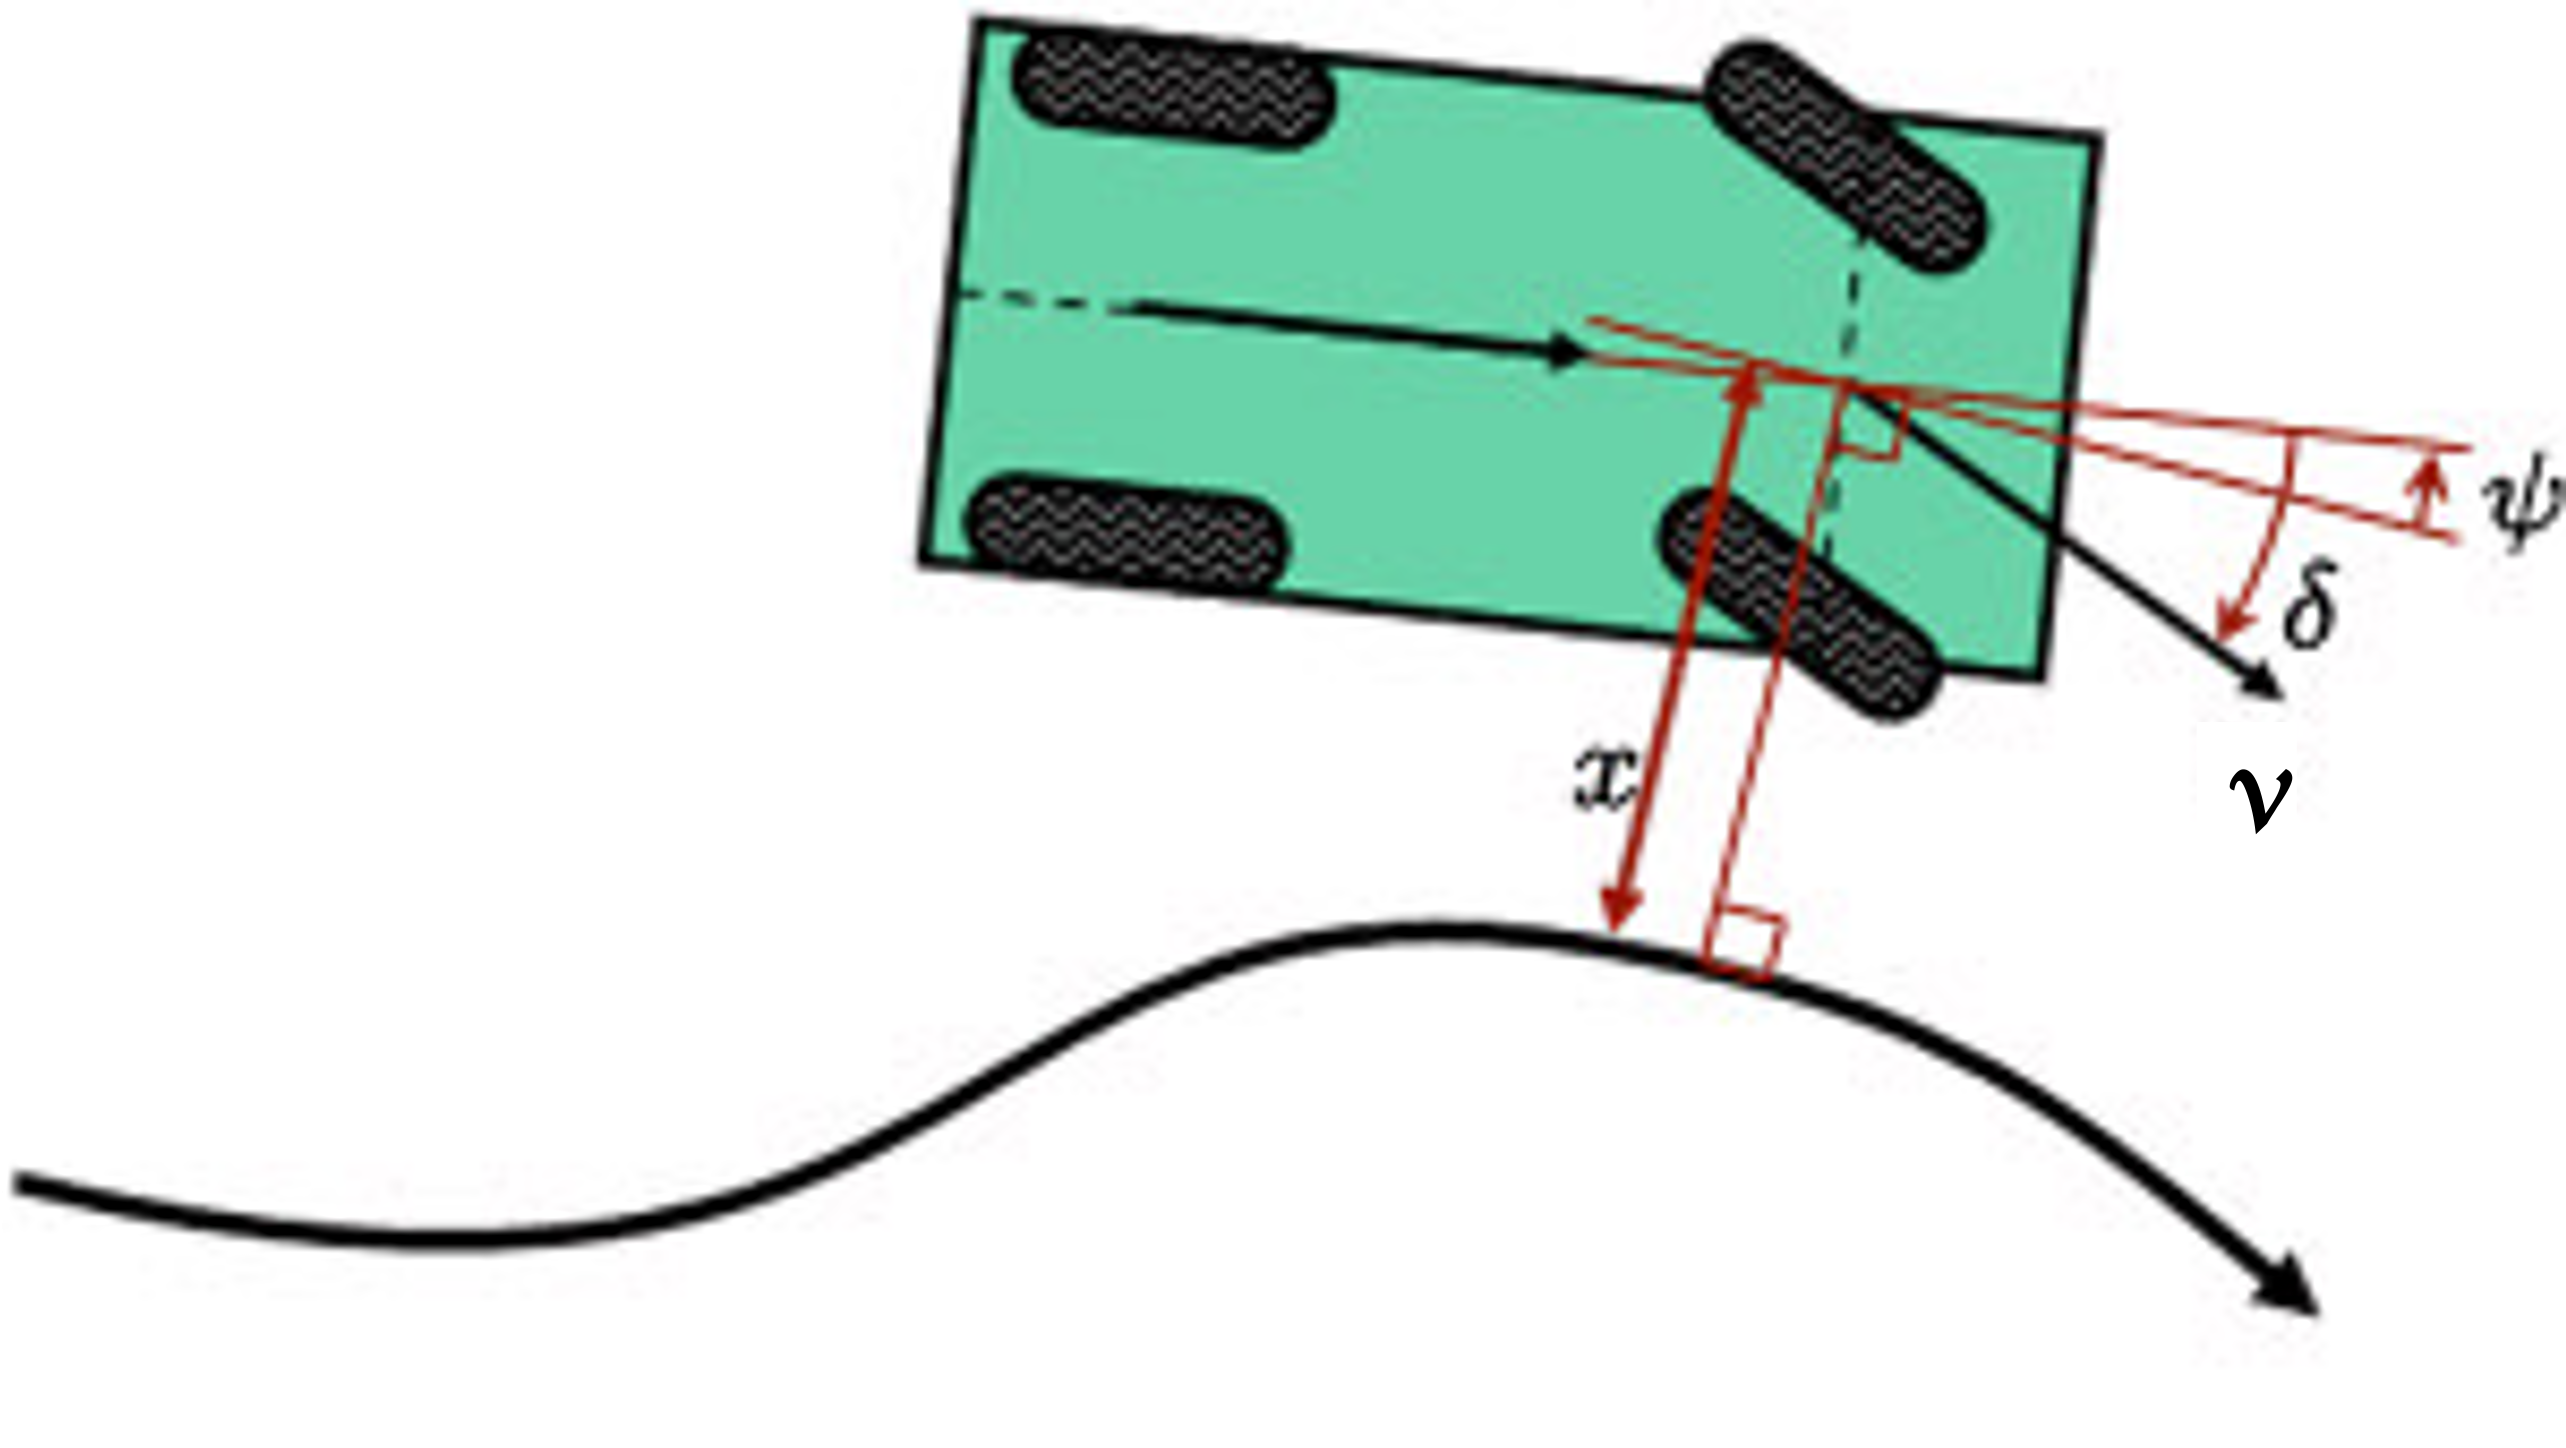
\includegraphics[width=0.5\linewidth]{Pictures/stanleySkizze.png}
    \caption{Stanley-Parameter}
    \cite{stanley_DARPA_grand_challange}
    \label{fig:stanley_parameter}
\end{figure}

Diese Parameter bilden, gemeinsam mit der aktuellen Fahrzeuggeschwindigkeit \(v(t)\) und einem freien Regelparameter \(k\), die Formel für die Berechnung des Soll-Lenkwinkels \(\delta(t)\): \cite{stanley_DARPA_grand_challange}

\begin{equation}
\label{stanley_equation}
\delta(t)=\psi(t)+arctan\frac{k \cdot x(t)}{v(t)}
\end{equation}

Die Grundidee und Funktionsweise dieser Formel sind wie folgt: Ein großer \gls{CTE} führt zu einem deutlichen Lenkeinschlag in Richtung der Solltrajektorie. Wenn das Fahrzeug nun diese Richtung einschlägt, resultiert dies in einem zunehmenden Winkelunterschied zu der Solltrajektorie \(\psi(t)\), welcher nun gegen den Lenkeinschlag des \gls{CTE} arbeitet. Mit Annäherung des Fahrzeuges an die Solltrajektorie wird der \gls{CTE} kleiner und \(\psi(t)\) bestimmt immer mehr den berechneten Soll-Lenkwinkel. Dies bewirkt, dass sich das Fahrzeug, wenn es sich nah an der Solltrajektorie befindet, in die gleiche Richtung wie die Solltrajektorie ausrichtet.

\subsection{Model Predictive Control}
\autor{Aaron J. Müller}
Einer der vielversprechendsten Ansätze der letzten Zeit, die Regelung von autonomen Fahrzeugen umzusetzen, ist \gls{MPC}.
Dabei ist festzuhalten, dass \gls{MPC} nicht ein konkreter Algorithmus, sondern eher eine Reglerfamilie ist.
Daher gibt es auch viele verschiedene Ansätze, \glspl{MPC} für autonome Fahrzeuge umzusetzen.

Die Idee der \gls{MPC} stammt ursprünglich aus den 1960er Jahren, in denen Lee und Markus ein iteratives Verfahren basierend auf einer Modellierung des offenen Regelkreises beschrieben \cite{lee1967foundations}.
Abbildung \ref{fig:MPC} zeigt den Aufbau eines \gls{MPC}-Reglers.
Ausgehend vom aktuell gemessenen Zustand wird eine diskrete Simulation der Regelstrecke verwendet, um die Auswirkungen verschiedener Eingabesignale zu testen.
Die Simulation wird bis zu einem zeitlichen Horizont durchgeführt, man spricht dabei auch von einem \enquote{Receding Horizon}.
Die simulierten Zustände werden mit einem Sollzustand verglichen und die Abweichungen in einer Kostenfunktion abgebildet.
Durch Minimierung dieser Kostenfunktion kann dann das optimale Eingabesignal bestimmt werden, welches bis zur nächsten Iteration angelegt wird.
Bemerkenswert ist, dass über die Kostenfunktion auch Rahmenbedingugen in den Regler eingebaut werden können, zum Beispiel Maximalwerte der Stellgrößen.

\begin{figure}[H]
    \centering
    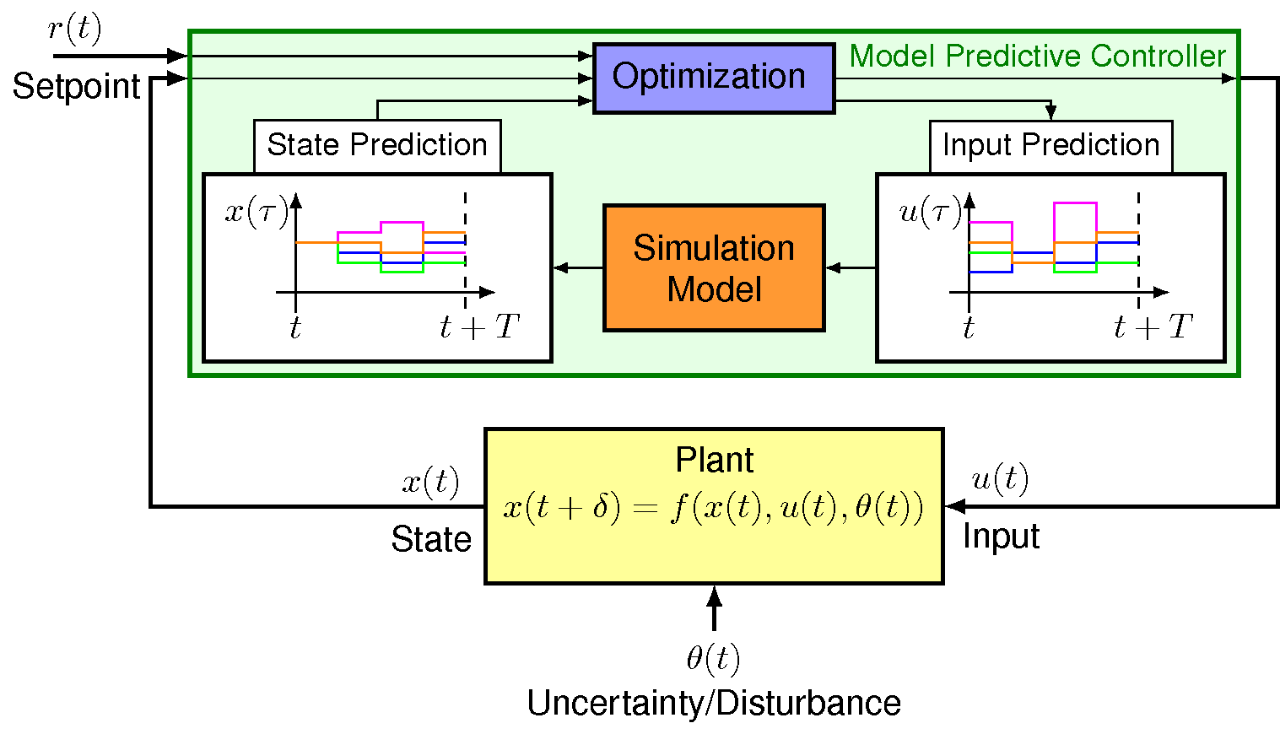
\includegraphics[width=0.75\linewidth]{Pictures/MPC_general.png}
    \caption{MPC Blockschaltbild}
    Quelle: \cite{mpc-uni-stuttgart}
    \label{fig:MPC}
\end{figure}

Die Entwicklung von \gls{MPC} wurde Anfangs vor allem durch die Industrie vorangetrieben \cite{qin1997overview}, beispielsweise in der Chemieverarbeitung oder in Kraftwerken. 
Im Kontext der Lateralregelung von selbstfahrenden Fahrzeugen taucht \gls{MPC} erstmals Anfang des 21. Jahrhunderts auf \cite{mpc-of-an-autonomous-vehicle}. 
Seitdem gibt es zahlreiche Weiterentwicklungen und Verbesserungen, welche verschiedene Herausforderungen der Entwicklung eines \gls{MPC}-basierten Lateralreglers lösen.
Ein prominentes Beispiel ist die Linearisierung des dynamischen Fahrzeugmodells, zum Beispiel durch Approximation mit Taylor-Reihen \cite{gao2021robust} oder durch Kombination mit Methoden des Maschinellen Lernens \cite{ilmpc}.

\newpage
\section{Design und Implementierung}
\subsection{Auswahl des Reglers}
\autor{Aaron J. Müller}
Im direkten Vergleich liefert \gls{MPC} ein deutlich besseres Regelverhalten als der Stanley Regler \cite{stanley_mpc_comparison1}\cite{stanley_mpc_comparison2}. 
Durch die Entscheidung, bei Hardwareupgrades eine hohe Rechenleistung zu präferenzieren, ist die aufwändigere Berechnung der Simulation und Optimierungsfunktion auch realisierbar.
Als weiteren Vorteil ist, dass eine \gls{MPC}-Regler auch als \gls{MIMO} System entworfen werden kann, um zusätzlich die Aufgabe der Longitudinalregelung zu übernehmen.
Dadurch könnte der bestehende Longitudinalregler im gleichen Schritt durch eine bessere Alternative ersetzt werden.

Entgegen dieser Vorteile wurde jedoch die Entscheidung getroffen, den Stanley-Regler umzusetzen. 
Der treibende Grund hierfür ist der vergleichsweise niedrige Entwicklungsaufwand, sowohl wegen der einfacheren Logik als auch wegen schon bereits bestehender Vorarbeit an einem Stanley-Regler für den it:movES Softwarestack \cite{Nico_Stanley}.
Die Implementierung des \gls{MPC} würde im Gegenzug den Fortschritt des Gesamtprojektes sabotieren, der aufgrund der Teilnahme an der \gls{BFMC} in einem festen Zeitplan gebunden ist.

\subsection{Solltrajektorie}
\autor{Aaron J. Müller}
Eine robuste Solltrajektorie ist essentiell für ein gutes Regelverhalten.
Auch wenn die Generierung der Solltrajektorie nicht direkt Teil der Entwicklung des Reglers ist, so muss doch ein geeignetes Interface definiert werden.
Die bisher verwendete Solltrajektorie stellt die Mitte der aktuell befahrenen Spur dar, und wird durch einen Offset von der Fahrbahnbegrenzung ermittelt.
Der bisherige Regler verwendet dann den \gls{CTE} und die Krümmung, um den Lenkwinkel zu berechnen.

Da der Stanley-Regler stattdessen koordinatenbasiert arbeitet, gibt es zwei mögliche Vorgehensweisen:
\begin{itemize}
    \item Der Regler erhält weiterhin eine parametrische Beschreibung der Trajektorie, und errechnet die benötigten Koordinaten selber
    \item Der Regler erhält die Solltrajektorie direkt als Reihe von Koordinatenpaaren
\end{itemize}

Bei einer kontinuierlichen Kurve kann die Referenzposition genauer gewählt werden.
Im Gegenzug ist die Verarbeitung von Koordinaten einfacher, was vor allem für die Transformation zwischen verschiedenen Koordinatensystemen von Bedeutung ist.

Ein weiterer wichtiger Punkt der berücksichtigt werden sollte, ist dass die Verwendung von Koordinatenpaaren eine flexiblere Berechnung des Sollgierwinkels ermöglicht, näheres dazu wird im späteren Abschnitt \ref{controller-gierwinkel} erläutert.
\newline
Aus den genannten Gründen wurde eine koordinatenbasierte Solltrajektorie gewählt, und als Schnittstelle definiert.
Es gilt noch zu untersuchen, ob die Berechnung der Solltrajektorie wie sie bisher implementiert ist auf Koordinatenpaare angepasst werden kann, oder ob diese durch Abtastung der parametrischen Kurve bestimmt werden müssen.
In beiden Fällen muss Rücksicht auf die Kameraperspektive genommen werden, sodass die errechneten Koordinatenpaare immer einen konstanten Abstand zueinander aufweisen.


\subsection{Sollgierwinkel}
\label{controller-gierwinkel}
\autor{Aaron J. Müller}
Für die Berechnung des Sollgierwinkels aus der Solltrajektorie gibt es grundsätzlich zwei anwendbare Formeln \cite{Nico_Stanley}, welche mit den beiden Darstellungen der Solltrajektorie korrelieren.

Allgemein lässt sich der Sollgierwinkel aus der Fahrgeschwindigkeit $v$ und der Krümmung der Solltrajektorie, $\kappa_{ref,W}$, berechnen (Formel \ref{sollgierwinkel_krümmung}).
Dabei ist zu beachten, dass die Krümmung an der gewählten Referenzposition verwendet wird. 
Es ist also ungünstig, die Krümmung der gesamten Trajektorie, so wie sie in der Parabeldarstellung der Solltrajektorie enthalten ist, zu verwenden.

\begin{equation}
\label{sollgierwinkel_krümmung}
\psi_{ref,W}=v\kappa_{ref,W}=\frac{v}{r_{ref,W}}
\end{equation}

Durch umformen lässt sich Formel \ref{sollgierwinkel_geschwindigkeiten} bilden, welche den Sollgierwinkel in Abhängigkeit der Geschwindigkeitskomponenten $\dot{x}_{ref,W}$ und $\dot{y}_{ref,W}$ berechnet.

\begin{equation}
\label{sollgierwinkel_geschwindigkeiten}
\psi_{ref,W}=\arctan \left( \frac{\dot{y}_{ref,W}}{\dot{x}_{ref,W}} \right)
\end{equation}

Diese Formel ist geeigneter, da die Geschwindigkeitskomponenten durch die partiellen Differenzialquotienten aus den Koordinaten der Punkte auf der Referenztrajektorie berechnet werden können.
Ein Vorteil dieser Art der Approximation ist, dass sie sehr flexibel ist.
Man kann so zum Beispiel die Differenzialquotienten über mehrere Intervalle bilden, und so Rauschen reduzieren.

\subsection{Vorschauweite}
\autor{Felix Anslinger}

Damit der Lateral-Regler erwartungsgemäß funktioniert, muss die Vorschauweite bei der Implementierung des Reglers beachtet werden. Der Grund hierfür lässt sich auf eine gewisse Verzögerung zurückführen, welche zwischen der Erfassung des Kamerabildes und dem Eintreffen der verarbeiteten Daten beim Regler besteht. Diese sogenannte Totzeit setzt sich aus verschiedenen Berechnungszeiten einzelner Softwarekomponenten zusammen und führt dazu, dass Punkte, die in einem aufgenommenen Kamerabild ursprünglich noch mit einer gewissen Distanz vor dem Fahrzeug lagen, nach der Verarbeitung dem Fahrzeug näher gerückt sind. Die Vorschauweite entspricht daher der Distanz, welche das Fahrzeug während der Totzeit zurücklegt.

Die Formel zur Berechnung dieser Vorschauweite ist simpel und ausschließlich abhängig von der Totzeit und der Geschwindigkeit des Fahrzeuges:

\begin{equation}
\label{vorschauweite_simpel}
D_{Preview} = v(t) \cdot T_{dead}
\end{equation}

Etwas komplexer wird es, wenn nun die Vorschauweite in Bezug auf das aufgenommene Kamerabild berechnet werden soll. Diese Berechnung ist zusätzlich abhängig von der Positionierung der Kamera an dem Fahrzeug und der Größe des Sichtfeldes. Sie lässt sich wie folgt berechnen:

\begin{equation}
\label{vorschauweite_kamerabild}
D_{Preview} = v(t) \cdot T_{dead} - tan(\alpha_{Camera} - \frac{\alpha_{POV}}{2}) \cdot h_{Camera} - X_{CameraOffset}
\end{equation}

Diese Formel bestimmt, wie viele Meter in dem Kamerabild vorausgeschaut werden muss, um den Punkt zu identifizieren, welcher sich nach der Totzeit auf Höhe des Fahrzeugs befindet. Die Beziehungen der einzelnen Variablen kann dem Schaubild \ref{fig:skizze_parameter_vorschauweite} entnommen werden.

\begin{figure}[H]
    \centering
    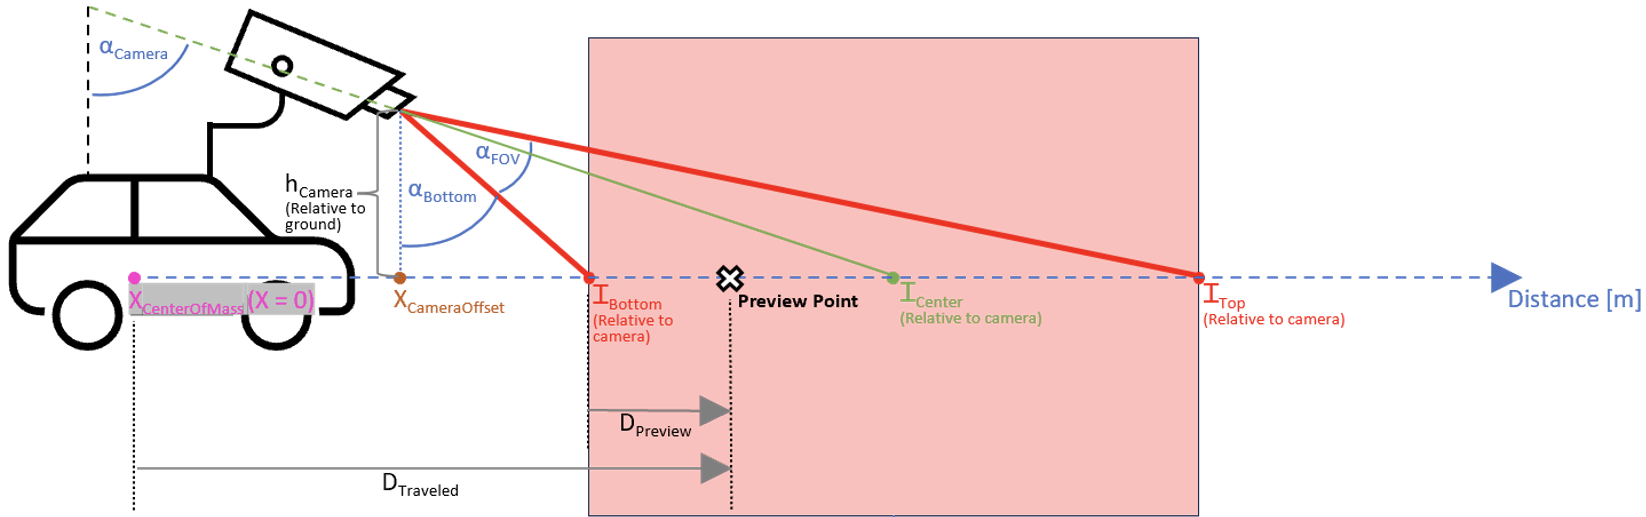
\includegraphics[width=1\linewidth]{Pictures/Bildschirmfoto 2024-02-05 um 01.49.52.png}
    \caption{Skizze der nötigen Parameter für die Berechnung der Vorschauweite}
    \label{fig:skizze_parameter_vorschauweite}
\end{figure}

Die Bestimmung der Vorschauweite ist jedoch mit der Einschränkung verbunden, dass sie nicht beliebig klein werden kann, da der untere Bildrand die minimale Vorschauweite vorgibt. Somit kann bei sehr langsamen Fahrten die Vorschauweite minimal auf die Distanz des unteren Bildrandes gesetzt werden. 


\subsection{Bestimmen von Parametern}
\autor{Felix Anslinger}

Das genaue Bestimmen von gewissen Parametern ist notwendig, damit der Regler bestmöglich funktionieren kann. Für die, in den vorherigen Kapiteln beschriebene, Implementierung des Stanley-Reglers, wird das genaue Bestimmen der Totzeit \(T_{dead}\), sowie der Montageposition der Kamera durch \(h_{Camera}\) und \(X_{CameraOffset}\), vorausgesetzt. 
Für das Bestimmen von solchen Parametern, empfiehlt es sich abzuwarten, bis alle finalen Hardwareänderungen an dem Fahrzeug vollbracht wurden. Andernfalls können sich die Parameter durch weitere Hardwareänderungen im Nachhinein ändern und müssten demnach erneut bestimmt werden.

\newpage
\section{Ergebnisse}
\autor{Felix Anslinger}

Die Formel zur Berechnung der Vorschauweite wurde durch eine Python Simulation verifiziert. \cite{vorschauweite_notebook}

Durch die Implementierung des Stanley-Controllers in einer MATLAB/Simulink Umgebung, mittels der in Kapitel 4.3 beschriebenen Formeln, lässt sich die Performance des Reglers testen. Die Simulation umfasst nicht nur die Stanley-Regelformel, sondern bezieht auch eine simulierte Totzeit sowie die entsprechende Berechnung der, in Kapitel 4.3.4 beschriebenen, Vorschauweite mit ein. Das Ergebnis der Simulation ist in Abbildung \ref{fig:stanley_matlab_simulationsergebniss} dargestellt, wobei die gestrichelte blaue Linie die Solltrajektorie und die rote Linie die Fahrstrecke des Fahrzeugs abbilden.

\begin{figure}[H]
    \centering
    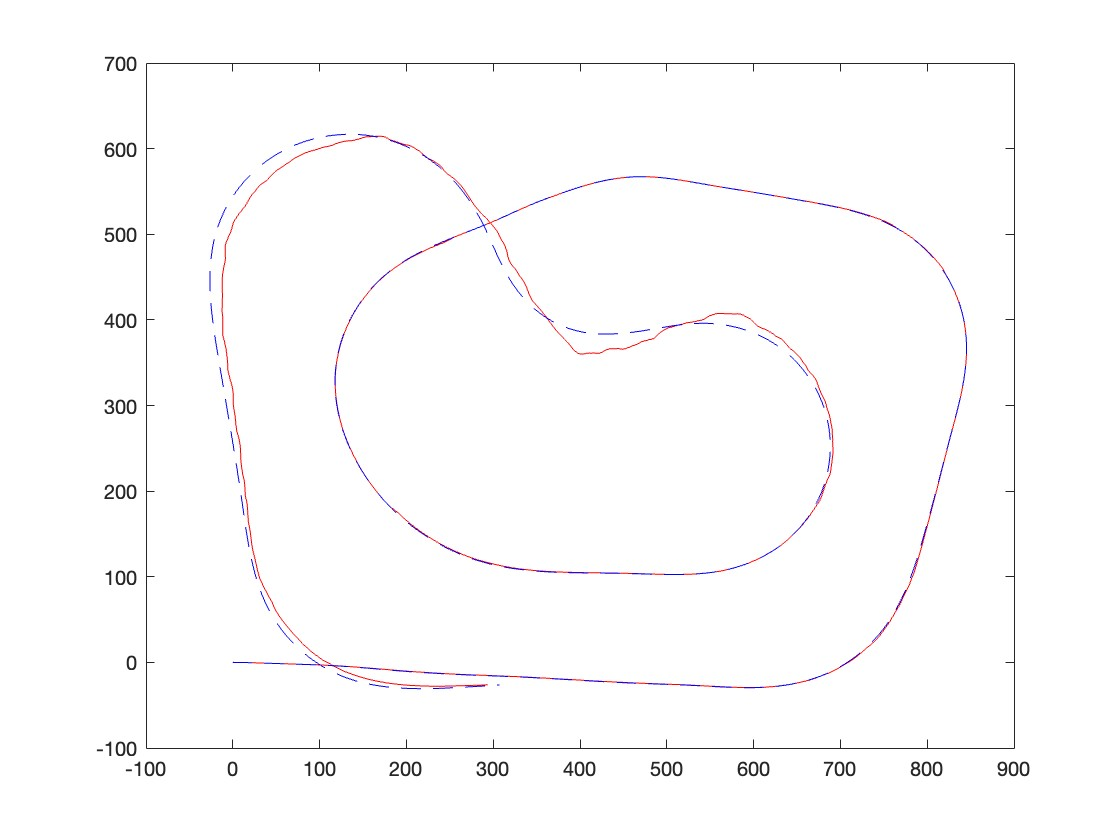
\includegraphics[width=1\linewidth]{Pictures/stanley_controller_performance_matlab.jpg}
    \caption{Stanley-Regler in MATLAB Simulation}
    \label{fig:stanley_matlab_simulationsergebniss}
\end{figure}

 Das Ergebnis aus Abbildung \ref{fig:stanley_matlab_simulationsergebniss} zeigt, dass der Stanley-Regler stabil ist und somit kein instabiles Aufschwingen auftritt. Des Weiteren lässt sich bei diesem Regler keine anhaltende Regelabweichung feststellen.


%\section{Ausblick}
\chapter{Behavior Tree}
\section{Einleitung und Motivation}
\autor{Medjen Izairi}
Autonomes Fahren, auch als selbstfahrende oder autonome Fahrzeugtechnologie bezeichnet, repräsentiert einen wegweisenden Fortschritt im Bereich der Mobilität. Bei dieser Technologie übernimmt das Fahrzeug die Steuerung, Navigation und oft auch die Entscheidungsfindung, ohne direkten menschlichen Eingriff. Im Zeitalter des autonomen Fahrens spielt die effiziente Steuerung des Verhaltens autonomer Fahrzeuge eine zentrale Rolle, um sichere und sozialverträgliche Interaktionen im Straßenverkehr zu gewährleisten. Die Herausforderung besteht darin, dass autonom agierende Fahrzeuge in Echtzeit komplexe Entscheidungen treffen müssen, um sich flexibel an wechselnde Verkehrssituationen anzupassen. In diesem Kontext gewinnen Verhaltensbäume (Behavior Trees) als ein flexibler und modularer Ansatz für die Entscheidungsfindung in autonom gesteuerten Systemen zunehmend an Bedeutung. Diese ermöglichen es, das Verhalten von autonomen Fahrzeugen auf eine übersichtliche und hierarchische Weise zu organisieren, was besonders in dynamischen und unvorhersehbaren Verkehrsszenarien von entscheidendem Vorteil ist. Das System kann in Echtzeitsituationen, in denen autonome Fahrzeuge sich schnell an veränderte Umgebungen anpassen müssen, effektiv und schnell auf neue Informationen reagieren Diese Fähigkeit erweist sich als entscheidend, insbesondere in Situationen mit hoher Sicherheitsrelevanz. In der bisherigen Softwarearchitektur wurde ein Switch Case (Fallunterscheidungen) als grundlegendes Entscheidungssystem verwendet. Obwohl das System anfangs funktional war, wies es einige Nachteile auf. Mit zunehmender Anzahl von möglichen Verhaltensszenarien stieg die Komplexität des Codes. Dies erschwerte nicht nur die Entwicklung, sondern auch die Wartung und Fehlerbehebung. In Echtzeitszenarien führte dies zu zahlreichen Verzögerungen und Schwierigkeiten, angemessen in Echtzeit zu reagieren. Daher haben wir uns für Behavior Trees entschieden, als eine effiziente Möglichkeit, die Komplexität unseres autonomen Fahrzeug-Systems zu bewältigen. 
\begin{figure}
    \centering
    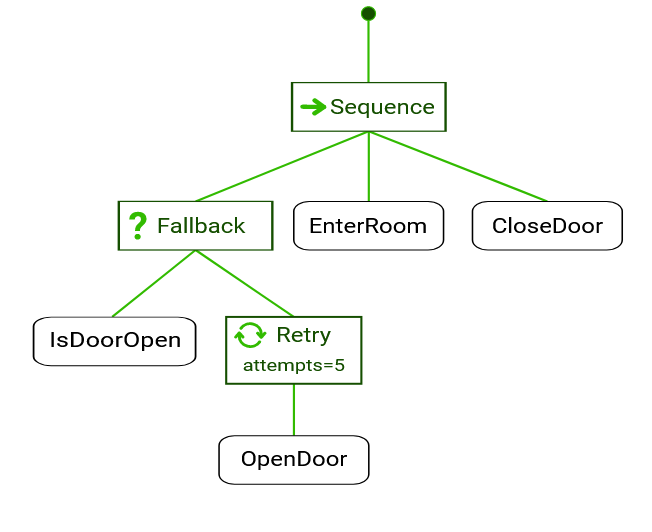
\includegraphics[width=0.45\linewidth]{Pictures/grafik.png}
    \caption{Behavior Tree}
    \cite{behaviortree}
    \label{fig:enter-label}
\end{figure}






\newpage
\section{Stand der Technik}
\autor{Medjen Izairi}
Für die Gestaltung und Anpassung der Behavior Tree in unserem Projekt verwenden wir Groot2, als eine fortschrittliche Software, die sich durch ihre benutzerfreundliche Drag-and-Drop-Oberfläche auszeichnet. Diese intuitive Benutzeroberfläche ermöglicht es Benutzern, Behavior Trees mühelos zu erstellen und zu bearbeiten, indem sie Knoten per Drag-and-Drop hinzufügen, verschieben und miteinander verbinden können.
Die Software erleichtert zudem die effiziente Verwaltung von umfangreichen Projekten durch die Unterstützung mehrerer Dateien. Diese Funktion ermöglicht es, den Überblick über komplexe Systeme zu behalten und die Arbeit an großen Verhaltensbaumprojekten zu optimieren.
\cite{groot2}\\

Eine weitere herausragende Funktion von Groot2 ist die Echtzeitvorschau des generierten XML-Codes des Behavior Trees. Die Funktion bietet einen klaren Überblick über die zugrunde liegende Struktur des Baums, wodurch die Entwicklungs- und Debugging-Prozesse optimiert werden. Insgesamt bietet Groot2 eine vielseitige und leistungsfähige Umgebung für die Entwicklung und Verwaltung von Behavior Tree, die sich durch Benutzerfreundlichkeit, Kompatibilität und erweiterte Funktionen auszeichnet.\cite{groot2}

\begin{figure}[H]
    \centering
    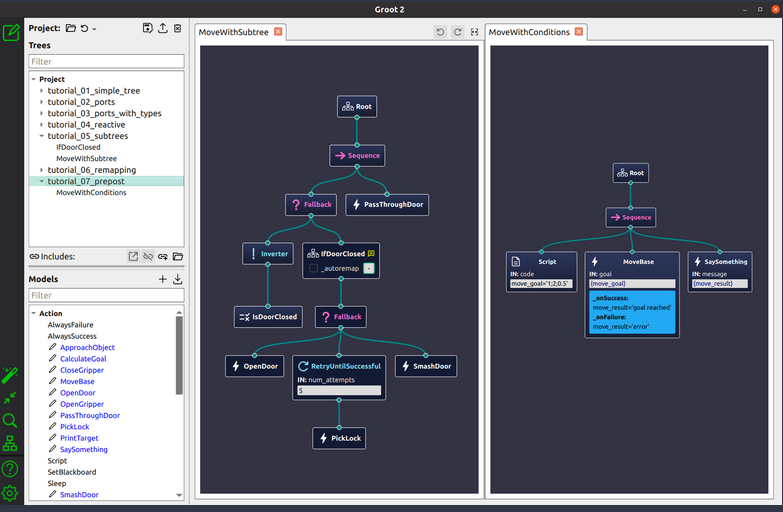
\includegraphics[width=0.85\linewidth]{Pictures/grafik2_groot2.png}
    \caption{Groot2}
    \cite{groot2}
\end{figure}



\newpage
\section{Design und Implementierung}
\autor{Gamze Isik}


\subsection{Werkzeuge}

Die Entscheidung für Groot2 als Tool für die Behavior-Tree-Implementierung in unserem autonomen Fahrsystem wurde durch seine benutzerfreundliche Oberfläche, die Flexibilität bei der Modellierung komplexer Verhaltensmuster und die nahtlose Integration in C++-Projekte getroffen. Die Integration erfolgt über .xml Dateien, die in C++ eingebunden werden. Diese .xml Dateien werden automatisch von Groot2 generiert.\\

Die Hauptmethode zur Überprüfung des Verhaltensbaums ist die Simulation innerhalb der Groot2-Benutzeroberfläche. Durch die Initiierung der Simulation kann der Verhaltensbaum in Echtzeit ausgeführt und visuell überwacht werden. Diese Methode ermöglicht eine detaillierte Analyse des Ablaufs des Verhaltensbaums, einschließlich der Aktivierung einzelner Knoten und der Reaktion des Fahrzeugs auf verschiedene Szenarien.\\

Als Bibliothek wird die Open-Source Library "BehaviorTree.CPP" verwendet. Diese C++-Bibliothek bietet ein Framework zur Erstellung von Verhaltensbäumen. Sie wurde entwickelt, um flexibel, benutzerfreundlich und schnell zu sein.\cite{bt-cpp}

\newpage
\subsection{Anforderungen und Szenarien}

Für die Konzeption des Verhaltensbaums werden die Anforderungen durch das BFMC definiert. Diese Anforderungen beziehen sich auf den Straßenverkehr und umfassen Szenarien, die das Fahrzeug beherrschen sollte, um die maximale Punktzahl zu erzielen. Dabei unterliegt das Fahrzeug einer Reihe von allgemeinen Verkehrsregeln:

\begin{itemize}
    \item Rechtsfahrgebot: Das Fahrzeug ist verpflichtet, auf der rechten Seite der Straße zu fahren, um den Verkehrsfluss und die Sicherheit zu gewährleisten.
    \item Überquerung von Linien: Gestrichelte Linien dürfen überquert werden, während durchgezogene Linien nicht überquert werden dürfen. Diese Regelung ist entscheidend für das korrekte Verhalten des Fahrzeugs im Straßenverkehr.
\end{itemize}

Darüber hinaus müssen spezifische Aktionen ausgeführt werden, sobald bestimmte Hindernisse auftreten:

\begin{table}[!h]
\centering
\begin{tabular}{ |p{4cm}|p{11cm}| }
\hline
\rowcolor{pink!35}
\textbf{Name} & \textbf{Beschreibung} \\
\hline
\cline{1-2}
Ampel & Begegnet vor der Kreuzung. Farbe ROT, das Fahrzeug muss halten. Grün, das Fahrzeug muss gehen, gelbe Farbe, bis zu Ihnen.\\
\cline{1-2}
Stopschild & Das Fahrzeug muss 3 Sekunden vor der Kreuzung anhalten.\\
\cline{1-2}
Zebrastreifen & Das Fahrzeug muss auf dem Fußgängerüberweg sichtbar abbremsen. \\
\cline{1-2}
Vorfahrt &  Das Fahrzeug muss ohne anzuhalten in die Kreuzung einfahren. \\
\cline{1-2}
Autobahneinfahrt & Das Fahrzeug muss seine Geschwindigkeit sichtbar erhöhen. \\
\cline{1-2}
Autobahnende & Das Fahrzeug muss wieder die normale Geschwindigkeit erreichen. \\
\cline{1-2}
Fußgänger auf dem Zebrastreifen & Der Fußgänger signalisiert die Absicht, die Straße am Zebrastreifen zu überqueren. Das Fahrzeug muss anhalten, bis die Aktion ausgeführt wird. \\
\cline{1-2}
Fußgänger auf nicht signalisierter Straße & Fußgänger, der sich in der Mitte der Fahrbahn befindet. Das Fahrzeug muss anhalten, bis die Straße frei ist.\\
\cline{1-2}
Feststehendes Fahrzeug & Feststehendes Fahrzeug simuliert falsches Parken oder eine Panne. Das Fahrzeug muss nach Möglichkeit überholen. \\
\cline{1-2}
Fahrendes Fahrzeug & Fahrendes Auto auf der Straße. Das Fahrzeug muss überholen, wenn es möglich ist, oder andernfalls hinterherfahren. \\
\cline{1-2}
Einbahnstraße & Signalisiert eine Einbahnstraße.\\
\cline{1-2}
Kreisverkehr & Signalisiert einen Kreisverkehr.\\
\cline{1-2}
Betreten verboten & Signalisiert eine nicht befahrbare Straße.\\
\cline{1-2}
\end{tabular}
\caption{Verkehrsregeln}
\cite{bfmc-traficRule}
\label{traficRules}
\end{table}

Beim Design des Behavior Trees fließen diese Anforderungen in die Konzeption mit ein.

\newpage
\subsection{Entwurf des Verhaltensbaums}

Bei der Gestaltung des Verhaltensbaums für das Fahrzeug werden die Anforderungen an die Echtzeit-Entscheidungsfindung sorgfältig berücksichtigt. Der hierarchisch strukturierte Behavior Tree beinhaltet verschiedene Ebenen von Entscheidungsprozessen, die eine präzise Steuerung des Fahrzeugs ermöglichen.\\

In Groot2 stehen unterschiedliche Arten von Knoten (Nodes) zur Verfügung, die sich ideal für die Modellierung von Verhaltensbäumen in autonomen Systemen eignen. Im Folgenden werden einige grundlegende Knotenarten vorgestellt, die in Groot2 verfügbar sind:

\begin{itemize}
    \item \textbf{Sequenzknoten}: Dieser Knoten führt seine Kinder nacheinander aus. Wenn ein Kindknoten fehlschlägt, wird die Ausführung abgebrochen.
    \item \textbf{Dekoratorknoten}: Dekoratorknoten verändern das Verhalten ihres Kindknotens. Beispiele sind Inverter (invertiert das Ergebnis des Kindknotens) oder Repeater (wiederholt die Ausführung).
    \item \textbf{Bedingungsknoten}: Dieser Knoten überprüft eine bestimmte Bedingung und gibt zurück, ob sie wahr oder falsch ist. Es wird oft in Verbindung mit Sequenz- oder Selektorknoten verwendet, um Entscheidungen zu treffen.
    \item \textbf{Aktionsknoten}: Aktionsknoten repräsentieren konkrete Aktionen oder Operationen, die im System ausgeführt werden sollen. Zum Beispiel das Navigieren zu einem bestimmten Punkt oder das Bremsen des Fahrzeugs.
    \item \textbf{Fallbacks}:
    \item \textbf{Wurzelknoten (Root)}: Dieser Knoten bildet den Einstiegspunkt des Verhaltensbaums. Je nach Konfiguration kann es sich um einen Sequenzknoten, Selektorknoten oder einen anderen Knotentyp handeln.
\end{itemize}

Diese Knoten kommen im Behavior Tree zum Einsatz, um die Struktur und Logik des Baums zu gestalten. An dieser Stelle ist es wichtig zu betonen, dass der Behavior Tree noch nicht abschließend ist und einige Anforderungen noch nicht vollständig erfüllt wurden. Aktuell wurden folgende Anforderungen im vorliegenden Stand des Behavior Trees umgesetzt:\\


\begin{itemize}
    \item Ampel
    \item Verkehrsschilder wie Stopschild, Vorfahrt, Zebrastreifen, Kreisverkehr
    \item Überholvorgang
    \item Fußgänger überquert den Zebrastreifen
    \item Ein Fahrzeug befindet sich im Kreisverkehr
    \item Autobahneinfahrt
    \item Autobahnausfahrt
    \item Einbahnstraße
    \item Betreten verboten
\end{itemize}

\newpage
\subsection{Implementierung}

Die Umsetzung der bereits festgelegten Punkte im Code erfolgt durch die Erstellung eines Code-Rumpfes, wobei jeder Knoten im Baum als eigene Funktion implementiert wird. Zur Veranschaulichung wird hier ein Code-Snippet für das Szenario eines Überholvorgangs erstellt. Damit die BehaviorTree.CPP Bibliothek verwendet werden kann, ist es notwendig, sie durch den Include-Befehl in den Code zu integrieren:

\begin{lstlisting}[language=C++, caption={Import der Bibliothek}]
#include <iostream>
#include <chrono>
#include "behaviortree_cpp/action_node.h"
#include "behaviortree_cpp/bt_factory.h"

\end{lstlisting}

Im nächsten Schritt werden die Bedingungsknoten in Funktionen umgewandelt. Dabei werden die Return-Statements in den Zeilen 7, 13 und 19 entsprechend bearbeitet, um den erfolgreichen Verlauf eines Überholvorgangs zu signalisieren. Hierbei wird SUCCESS zurückgegeben:

\begin{lstlisting}[language=C++, caption={Bedingungsknoten}]
using namespace std::chrono_literals;

//CarInFront subtree
BT::NodeStatus CarInFront()
{
    std::cout << "Car is in front" << std::endl;
    return BT::NodeStatus::SUCCESS;
}

BT::NodeStatus solidLane()
{
    std::cout << "Overtake allowed" << std::endl;
    return BT::NodeStatus::SUCCESS;
}

BT::NodeStatus Gegenverkehr()
{
    std::cout << "No incoming traffic" << std::endl;
    return BT::NodeStatus::SUCCESS;
}
\end{lstlisting}

\newpage
Die Aktionsknoten werden nun in Form von Klassen implementiert. Im Folgenden sind die Klassen Overtake, Stop und Cruise als eigenständige Klassen umgesetzt, wodurch sie für die Wiederverwendung bereitstehen. Durch die Anpassungen des Szenarios, welches auf einen möglichen Überholvorgang ausgelegt ist, geben die Klassen Overtake und Cruise SUCCESS zurück:

\begin{lstlisting}[language=C++, caption={Aktionsknoten}]
class Overtake : public BT::SyncActionNode
{
    public:
        explicit Overtake(const std::string &name) : BT::SyncActionNode(name, {})
        {
        }
    BT::NodeStatus tick() override
    {
        std::this_thread::sleep_for(3s); //overtaking phase not longer than 2 minutes
        std::cout << "Overtook car" << std::endl;
        return BT::NodeStatus::SUCCESS;
    }
};

class Stop : public BT::SyncActionNode
{
    public:
        explicit Stop(const std::string &name) : BT::SyncActionNode(name, {})
        {
        }
    BT::NodeStatus tick() override
    {
        std::cout << "Car stopped" << std::endl;
        return BT::NodeStatus::FAILURE;
    }
};

class Cruise : public BT::SyncActionNode
{
    public:
        explicit Cruise(const std::string &name) : BT::SyncActionNode(name, {})
        {
        }
    BT::NodeStatus tick() override
    {
        std::cout << "Cruise" << std::endl;
        return BT::NodeStatus::SUCCESS;
    }
};
\end{lstlisting}

\newpage
Um den Code auszuführen, ist es erforderlich, die einzelnen Bedingungsknoten, Aktionsknoten und Knotentypen zu registrieren. Im Anschluss wird in Zeile 15 die zuvor in Groot2 erstellte .xml-Datei integriert. Diese Datei enthält die strukturelle Darstellung des Baums:

\begin{lstlisting}[language=C++, caption={Ausführen des Codes - main()}]
int main()
{
    BT::BehaviorTreeFactory factory;

    factory.registerSimpleCondition("CarInFront", std::bind(CarInFront));
    factory.registerSimpleCondition("solidLane", std::bind(solidLane));
    factory.registerNodeType<Overtake>("Overtake");

    factory.registerSimpleCondition("Gegenverkehr", std::bind(Gegenverkehr));

    factory.registerNodeType<Stop>("Stop");
    factory.registerNodeType<Cruise>("Cruise");

    //create tree
    auto tree = factory.createTreeFromFile("./../BFMC_24.xml");

    tree.tickOnce();

    return 0;
}

\end{lstlisting}









\newpage
\newpage
\section{Ergebnisse}
\autor{Gamze Isik}

Bei Ausführung des Codes für den Überholvorgang ergibt sich folgende Ausgabe:

\begin{lstlisting}[language=bash, caption={Ausgabe - Überholvorgang}]
Car is in front
Overtake allowed
No incoming traffic
Overtook car
\end{lstlisting}

Dies deutet darauf hin, dass die Logik für den Überholvorgang erfolgreich umgesetzt wurde und das Fahrzeug sich gemäß den vorgesehenen Plänen verhalten hat.\\

\textbf{XML Datei}

Die XML Datei entspricht der Abbildung \ref{fig:bt_bfmc24} in textueller Form. Dabei ist es wichtig zu beachten, dass die Funktionsnamen mit den Namen der entsprechenden Knoten übereinstimmen müssen, um eine korrekte Erkennung zu gewährleisten.

\begin{lstlisting}[language=xml, caption={Behavior Tree - XML Struktur}]
<?xml version="1.0" encoding="UTF-8"?>
<root BTCPP_format="4"
      main_tree_to_execute="BFMC_24">
  <BehaviorTree ID="BFMC_24">
    <Fallback>
      <Sequence>
        <CarInFront/>
        <Fallback>
          <solidLane/>
          <Stop/>
        </Fallback>
        <Fallback>
          <Gegenverkehr/>
          <Stop/>
        </Fallback>
        <overtake/>
      </Sequence>
      <Sequence>
        <stopLine/>
        <slowDown/>
        <Fallback>
          <Sequence>
            <Schild/>
            <slowDown/>
            <Fallback>
              <Sequence>
                <Stoppschild/>
                <Stop/>
                <Delay delay_msec="3000">
                  <Cruise/>
                </Delay>
              </Sequence>
              <Sequence>
                <Priority/>
              </Sequence>
              <Sequence>
                <Crosswalk/>
                <stopLine/>
                <slowDown/>
                <Fallback>
                  <PedestrianOnCrosswalk/>
                  <Precondition else="FAILURE"
                                if="noPedestrian">
                    <KeepRunningUntilFailure>
                      <Stop/>
                    </KeepRunningUntilFailure>
                  </Precondition>
                  <Cruise/>
                </Fallback>
              </Sequence>
              <Sequence>
                <RoundAbout/>
                <slowDown/>
                <Fallback>
                  <CarInRoundAbout/>
                </Fallback>
                <Precondition else="FAILURE"
                              if="!auto">
                  <KeepRunningUntilFailure>
                    <Stop/>
                  </KeepRunningUntilFailure>
                </Precondition>
                <accelerate/>
              </Sequence>
            </Fallback>
          </Sequence>
          <Sequence>
            <trafficLight/>
            <slowDown/>
            <Fallback>
              <Sequence>
                <redOrYellowLight/>
                <Stop/>
              </Sequence>
              <Sequence>
                <greenLight/>
              </Sequence>
            </Fallback>
          </Sequence>
        </Fallback>
        <Sequence>
          <HighwayEntry/>
        </Sequence>
        <Sequence>
          <HighwayEnd/>
          <slowDown/>
          <normalSpeed/>
        </Sequence>
        <Sequence>
          <OneWay/>
        </Sequence>
        <Sequence>
          <NoEntry/>
          <Stop/>
        </Sequence>
        <accelerate/>
      </Sequence>
      <Cruise/>
    </Fallback>
  </BehaviorTree>

  <!-- Description of Node Models (used by Groot) -->
  <TreeNodesModel>
    <Condition ID="CarInFront"
               editable="true"/>
    <Condition ID="CarInRoundAbout"
               editable="true"/>
    <Condition ID="Crosswalk"
               editable="true"/>
    <Action ID="Cruise"
            editable="true"/>
    <Condition ID="Gegenverkehr"
               editable="true"/>
    <Condition ID="HighwayEnd"
               editable="true"/>
    <Condition ID="HighwayEntry"
               editable="true"/>
    <Condition ID="NoEntry"
               editable="true"/>
    <Condition ID="OneWay"
               editable="true"/>
    <Condition ID="PedestrianOnCrosswalk"
               editable="true"/>
    <Condition ID="Priority"
               editable="true"/>
    <Condition ID="RoundAbout"
               editable="true"/>
    <Condition ID="Schild"
               editable="true"/>
    <Action ID="Stop"
            editable="true"/>
    <Condition ID="Stoppschild"
               editable="true"/>
    <Action ID="accelerate"
            editable="true"/>
    <Condition ID="greenLight"
               editable="true"/>
    <Action ID="normalSpeed"
            editable="true"/>
    <Action ID="overtake"
            editable="true"/>
    <Condition ID="redOrYellowLight"
               editable="true"/>
    <Action ID="slowDown"
            editable="true"/>
    <Condition ID="solidLane"
               editable="true"/>
    <Condition ID="stopLine"
               editable="true"/>
    <Condition ID="trafficLight"
               editable="true"/>
\end{lstlisting}

Aktuell befindet sich sowohl die Datei als auch die folgende Abbildung \ref{fig:bt_bfmc24} in einem Prozess der Erweiterung und Verbesserung, um sicherzustellen, dass die maximale Punktzahl im Rahmen des \gls{BFMC} erreicht werden kann.

\newpage
\textbf{Behavior Tree Struktur}

\begin{figure}[!h]
    \centering
    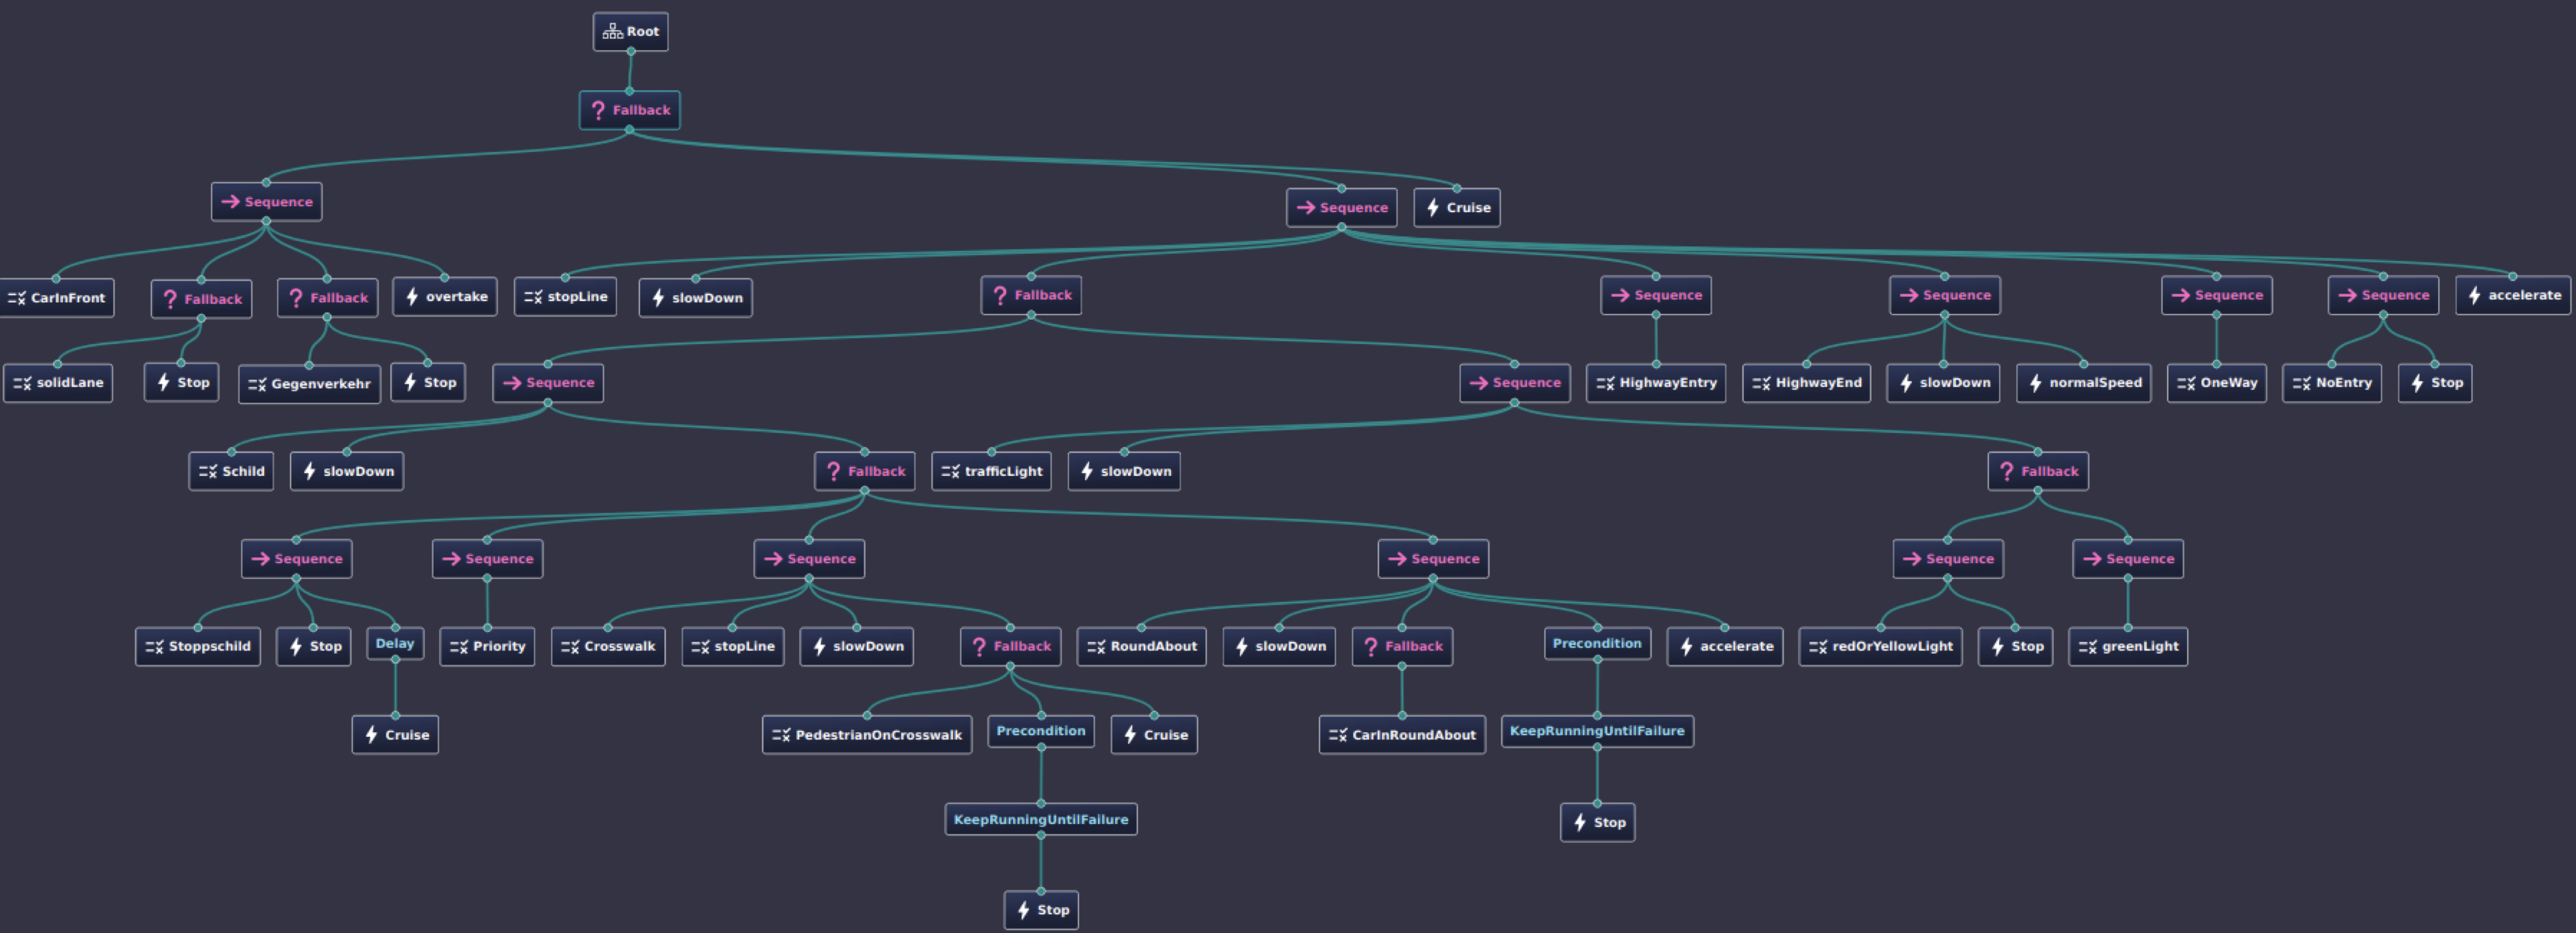
\includegraphics[width=1.4\linewidth, angle=90]{Pictures/behavior_tree_groot2.png}
    \caption{Behavior Tree für die \gls{BFMC} 2024}
    \label{fig:bt_bfmc24}
\end{figure}




\newpage
\section{Ausblick}
\autor{Gamze Isik}

Aspekte, die bisher noch nicht in Betracht gezogen wurden, umfassen beispielsweise die Interaktion mit Fußgängern auf nicht signalisierten Straßen. Des Weiteren steht die Integration des Behavior Trees in den it:movES Software Stack noch aus. Dabei wird die Logik getestet, indem das Fahrzeug Hindernisse erfolgreich bewältigen soll. Im gegenwärtigen Code-Rumpf werden vorläufig SUCCESS oder FAILURE zurückgegeben, wobei die eigentliche Software-Stack-Logik noch nicht implementiert ist. Diese muss durch die entsprechenden Funktionen ersetzt werden, welche dem Fahrzeug durch die Publisher die erforderlichen Daten übermitteln. Dabei handelt es sich um Informationen darüber, ob das Fahrzeug weiterfahren, beschleunigen, verlangsamen, umlenken oder komplett stoppen soll.
\chapter{Diskussion}

In diesem Kapitel werden die Kalkulations-, und Messergebnisse der Performance analysiert und interpretiert. Anschließend wird der Prototyp bewertet und dabei auf dessen Grenzen eingegangen.
  
\section{Analyse und Interpretation der Ergebnisse}

Basierend auf der Kostenanalyse und den Ergebnissen der Kalkulation ergibt sich, dass die Speicherklassen OneZone-IA von AWS und Coldline von GC die niedrigsten Kosten für die Speicherung von Daten aufweisen. Jedoch sind Datenabrufe in diesen Speicherklassen als kostenintensiv zu betrachten. In der Coldline-Klasse belaufen sich die Kosten für Klasse A-, und B-Operationen jeweils auf 4,84 Euro, während bei AWS PUT-Anfragen, die mit Klasse A gleichzusetzen sind, 2,50 Euro und GET-Anfragen, die mit Klasse B gleichzusetzen sind, 0,50 Euro betragen. Insgesamt sind die Kosten für die Coldline-Klasse im Vergleich zur OneZone-IA-Klasse jedoch günstiger.\\ 

Die Entscheidung für OneZone-IA als Speicherklasse birgt das Risiko auf die Nicht-Verfügbarkeit von Daten bei Ausfall der AZ, da die Daten nur in einer Verfügbarkeitszone gespeichert werden. Dies steht im Widerspruch zu den Anforderungen von leoticket an eine hohe Verfügbarkeit. Obwohl die Speicherkosten in dieser Klasse am niedrigsten sind, sind die Kosten für Datenabrufe im Vergleich zu anderen Speicherklassen höher. Für leoticket ist es jedoch von Bedeutung, auf Objekte mindestens zweimal zugreifen zu können und sie den Kunden zur Verfügung zu stellen. Bei älteren Daten, die mehrere Jahre zurückliegen, kann es ratsam sein, die Objekte in S3 Glacier Instant Retrieval oder in GC Archive Storage zu verschieben, um Kosten für die Archivierung einzusparen und die Daten in Bereichen von Millisekunden zur Verfügung stehen können.\\

Die Verfügbarkeit der Coldline-Klasse ähnelt der OneZone-IA-Klasse. Die Datenabrufe in dieser Klasse können mehrere Stunden dauern. Sie ist nicht für Szenarien geeignet, die einen sofortigen Zugriff auf Daten erfordern oder in denen häufiger auf die Daten zugegriffen werden muss. Im Gegensatz zur OneZone-IA ist die Coldline-Klasse jedoch nicht auf eine einzelne Verfügbarkeitszone beschränkt. Aufgrund ihrer geringeren Kosten und der Verfügbarkeit in mehreren Availability Zones ist Coldline die bessere Option für die langfristige Archivierung von Daten. Da die Kosten für Datenabrufe in dieser Klasse höher sind als in allen anderen Speicherklassen, ist sie nicht geeignet für Daten, auf die mehr als einmal zugegriffen werden muss.\\

Im Rahmen der Performance-Analyse zeigte die OneZone-IA-Klasse eine bessere Leistung als die Coldline-Klasse. Bereits beim Upload von zehn Dateien war die OneZone-IA-Klasse deutlich schneller. In diesem Szenario war sie 20.6\% schneller wie die Coldline-Klasse. Beim Upload von 100 Dateien wurde ein Unterschied von 63\% festgestellt, wobei die Coldline-Klasse etwa 20 Sekunden und die OneZone-IA-Klasse nur etwa sieben Sekunden benötigte. Bei 1000 Dateien bewegten sich beide Speicherklassen im Minutenbereich, wobei auch hier die OneZone-IA-Klasse 55.34\% schneller wie die Coldline-Klasse war. Beim Download von Dateien bewegten sich beide Klassen in Millisekunden Bereichen. Ab 1000 Dateien war die Coldline-Klasse ungefähr 55\% langsamer als die OneZone-IA-Klasse.\\

Die Speicherklassen Standard-IA und Nearline weisen bei den Speicherkosten nur geringfügige Preisunterschiede  auf, die sich auf maximal zwei Euro belaufen. Dabei ist Nearline maximal zwei Euro günstiger als Standard-IA. Die Standard-IA eignet sich für seltene Datenabrufe, die jedoch eine schnellere Zugriffszeit erfordern, wenn sie benötigt werden. Die Nearline-Klasse ähnelt der Standard-IA und ist ebenfalls für Daten gedacht, die gelegentlich im Zeitraum von Wochen oder Monaten abgerufen werden. Sie ist ideal für Datensicherung, Datenmigration und Datenarchivierung. Beide Speicherklassen bieten einen Kompromiss zwischen Kosteneinsparungen und Datenzugriffszeiten.\\

Während der Performance Analyse wurden diese beiden Speicherklassen verglichen, da sie ähnliche Eigenschaften aufweisen. Es stellte sich heraus, dass sich die Dauer des Uploads und Downloads erst ab 10 Dateien zu unterscheiden began. Dabei war die Standard-IA beim Hochladen und Herunterladen der zehn Dateien fast dreimal so schnell wie die Nearline-Klasse. Die Nearline-Klasse schnitt beim Hochladen schlechter ab. Beim Herunterladen von Dateien gab es jedoch nur minimale Unterschiede, wobei die Nearline bei 1000 Dateien 61.55\% langsamer war wie die Standard-IA.\\

Die Standardklassen beider Anbieter weisen kaum Unterschiede bei den PUT- und GET-Anfragen auf. Allerdings sind die Speicherungskosten in der Standardklasse von AWS 9.27\% höher als bei GC. Beide Klassen eignen sich für Daten, auf die häufig zugegriffen wird und die eine hohe Verfügbarkeit, schnelle Zugriffszeiten und geringe Latenzzeiten erfordern. Beide Standardklassen sind für den allgemeinen Gebrauch optimiert, wobei die Speicherungskosten in diesen Klassen im Vergleich zu anderen Speicherklassen am höchsten sind.\\

Bei der Performance-Analyse schnitt die Standardklasse von AWS ab zehn Dateien etwa 54.4\% besser ab als die entsprechende Klasse von GC. Beim Hochladen von 100 Dateien war die AWS-Standardklasse etwa 60.9\% schneller und bei 1000 Dateien etwa 58\% schneller wie die GC Standardklasse. Beim Herunterladen von Dateien waren die Unterschiede nicht groß genug, um eine eindeutige Aussage über die Überlegenheit einer Klasse zu treffen. Allerdings war die AWS-Standardklasse bei 1000 Dateien etwa 60\% schneller.\\

Es ist anzumerken, dass bei den AWS Kosten auch die Vorabzahlung der Speicherung aller Objekte enthalten ist. Bei GC gibt es hingegen keine Vorabzahlung für die Speicherung von Objekten. Aus diesem Grund und auch durch die niedrigeren Gebühren der Speicherung ist GC die kostengünstigere Datenspeicherung.\\

Insgesamt war die Dauer des Uploads und Downloads der Speicherklassen von AWS in der Performance-Analyse niedriger als bei GC. Ab einer Datei traten bereits erste Unterschiede auf, wobei GC mehr Zeit in Anspruch nahm. Die Performance-Messungen basieren jedoch lediglich auf groben Schätzungen innerhalb einer virtuellen Umgebung, die von Hetzner Cloud bereitgestellt wurde. Hier ist anzumerken, dass der Hetzner Server näher am AWS Server liegen und deshalb bessere Ergebnisse in der Performance als GCP erzielen kann. Faktoren wie die Auslastung des Netzwerks können die Ergebnisse beeinflussen und stellen keine aussagekräftigen Performance-Ergebnisse dar.\\

\section{Bewertung des Prototyps}

Für die Bewertung des Prototyps wurden die Anforderungen von leoticket herangezogen. Dabei war es wichtig, den Prototypen so zu bauen, dass die sichere Speicherung gedeckt war. Für die Deckung der sicheren Speicherung wurden verschiedene Methoden betrachtet, die beide Cloud Provider anboten. Dabei implementiert der Prototyp die SSE-KMS Methode beider Provider. Durch die eigene Erstellung des Schlüssels in der KMS von AWS und GC hat der Nutzer mehr Kontrolle, da die Schlüssel von ihm selbst erstellt werden. Der Schlüssel wird vom KMS gespeichert und muss daher nicht vom Nutzer extern gespeichert und verwaltet werden. Der Prototyp kann jedoch so umgebaut werden, dass auch eine andere Methode wie die SSE-C verwendet werden kann. Die SSE-C bietet eine höhere Sicherheit, da der Nutzer den Schüssel selbst generieren und speichern muss. Dies führt aber auch zum Risiko, den Schlüssel zu verlieren. In diesem Fall kann auf die Objekte im Bucket nicht mehr zugegriffen werden. Noch ein Kriterium von leoticket war die hohe Verfügbarkeit der Daten. Der Prototyp wurde so gebaut, dass der Nutzer die Speicherklasse für AWS selbst wählen kann. In GC funktioniert das, indem das Bucket die richtige Speicherklasse bereits eingestellt hat. Für die Verfügbarkeit sind jedoch die Cloud Provider verantwortlich. Hier versprechen beide Provider eine Verfügbarkeit von mindestens 99.5\%. Diese Verfügbarkeit hängt von den verschiedenen Speicherklassen ab. Über Terraform werden Buckets automatisch mit den Einstellungen konform zu den Anforderungen von leoticket erstellt. Diese beinhalten die Konfigurationen von:

\begin{itemize}
	\item Object Versioning
	\item Lifecycle Rules
	\item Object Ownership
	\item Data Encryption
	\item Object Logging
	\item Bucket ACL
	\item Public Access Block
\end{itemize}

Die Objekt Versionierung dient zur Steigerung der Verfügbarkeit, falls Daten unerwünscht gelöscht oder überschrieben werden. Für die Anforderung der Integration in Software-Produkte wie leoticket sorgen die SDKs der beiden Provider. Diese unterstützen verschiedene Programmiersprachen. Sie werden durch Spring Boot unterstützt und können auch mit Maven oder Gradle gebaut werden. Die Anbindung verläuft gemäß der offiziellen Dokumentation der beiden Cloud Provider. Die Dokumentationen sind verständlich und auf dem aktuellsten Stand und beschreiben deren API. AWS und GC bieten auch neue Versionen an und updaten die SDKs. Die Generierung der signierten URLs ist für die Bereitstellung der Dateien zuständig. Diese Anforderung war das Hauptmerkmal von leoticket. Dabei ist es bei beiden Providern möglich, signierte, zeitlich begrenzte URLs zu generieren und diese Nutzern bereitzustellen. Empfänger der URL können so ihre Tickets und Rechnungen herunterladen. Für die Performance Analyse wird eine Methode zur Verfügung gestellt, die Testdateien in der Größe von 100 KB erstellen und in Buckets hoch- und herunterladen kann.\\

Insgesamt ist der Prototyp ausbaufähig und stellt für diese Arbeit einen Vergleich zwischen beiden Cloud Providern dar. Für den besseren Vergleich beider Cloud Provider wurden die Technologien ausprobiert und genutzt. Durch Änderungen an der Terraform Konfiguration, der Speicherklassen Variable für AWS und an der Methode der Datenverschlüsselung kann der Prototyp angepasst werden. Eine Schwäche des Prototyps besteht darin, dass keine genauen Performance Messungen durchgeführt werden können aufgrund genannter Einflüsse, welche die Ergebnisse beeinflussen können. Er dient lediglich dem groben Vergleich. Eine weitere Schwäche des Prototyps besteht darin, dass Entwickler bei der Integration des Prototyps in eigenen Anwendungen Anpassungen durchführen müssen, indem die Hauptklasse des Prototyps so umgebaut werden muss, dass sie dem gewünschten Verhalten entspricht.
\chapter{Fazit}

In diesem Kapitel werden die zuvor gestellten Fragen beantwortet. Darüber hinaus wird die potenzielle Anwendung des Prototyps diskutiert.

\section{Beantwortung der Forschungsfrage}

Folgende Fragen wurden am Anfang gestellt:

\begin{itemize}
	\item Welches Speichersystem ist im Hinblick auf Kosten, Performance und Verfügbarkeit für die Persistenz von Binärdaten besonders geeignet? 
	\item Wie können Daten durch sichere, zeitlich begrenzte URLs bereitgestellt werden?
\end{itemize}

Um die erste Frage zu beantworten, werden die Punkte des theoretischen Teils aufgegriffen. Es wurden verschiedene Speicherarten wie Objekt-, Block-, und File Storage untersucht. Dabei stellte sich heraus, dass Objekt Storage als Speichersystem für die Anforderungen von leoticket geeignet ist. Einige Cloud Provider stellen Objekt Storage zur Speicherung von Daten zur Verfügung und sind im Markt stark vertreten. Es wurden die zwei größten Cloud Provider AWS und GCP betrachtet und eine Vergleichsbasis hergestellt im Hinblick auf Kosten, Performance, Verfügbarkeit, Sicherheit, Bereitstellung der Daten und API Anbindungen. Bei der sicheren Speicherung war es wichtig, dass die Daten vertraulich gespeichert werden und nur Berechtigte Zugriff auf sie haben.\\

 Datenverschlüsselungsmethoden wurden bei beiden Cloud Providern betrachtet und dabei festgestellt, dass die SSE C zwar die stärkste unabhängige Sicherheit bietet, jedoch das Risiko besteht, selbstverwaltete und gespeicherte Schlüssel zu verlieren. Außerdem müssten Mitarbeiter dafür geschult werden, was extra Aufwand bedeutet. Aus diesem Grund wurde für die Implementierung des Prototyps die SSE-KMS customer-managed Methode verwendet, damit der Nutzer die Schlüssel in der KMS von den Providern selbst erstellen und verwalten kann. So bleibt die Kontrolle erhalten und verschafft höhere Sicherheit. Je nach den gewählten Speicherklassen versprechen beide Anbieter eine Verfügbarkeit von mindestens 99.5\%. Bei der Untersuchung der Speicherklassen in Verbindung mit Kosten und Performance stellte sich heraus, dass die Standard-IA von AWS und die Nearline von GC besser zu den Anforderungen von leoticket passen. Da die Latenz für leoticket kein Kriterium darstellt und vernachlässigt werden kann, fallen die Standard Klassen beider Provider weg. Die Standardklassen bieten zwar eine leistungsfähige Speicherlösung, jedoch gehen die eingesetzten Mittel über das hinaus, was tatsächlich benötigt wird. Da Daten über einen Zeitraum von bis zu zehn Jahren gespeichert werden müssen, sind die Speicherkosten für die Standardklassen im Vergleich zu anderen Optionen zu hoch. Die Speicherung der Daten auf längerer Sicht steht mehr im Fokus, da auf eine Datei im Durschnitt nur zweimal zugegriffen wird. Die OneZone-IA fällt ebenfalls weg, da die Daten nur in einer Availability Zone gespeichert werden. Das Risiko ergibt sich durch Nicht-Verfügbarkeit der Daten durch Speicherung in lediglich einer Zone. Daten müssen auf Abruf schnell zugreifbar sein, deshalb sind die OneZone-IA und die Coldline nicht geeignet, da sie eher für selten abgerufen Daten angepasst sind. Die Abrufkosten dieser Speicherklassen sind am höchsten und nicht zu empfehlen.\\

Insgesamt wird für die Persistenz von Binärdaten ein Object Storage mit den Speicherklassen Standard-IA von AWS und Nearline von GC empfohlen. Sie bieten die nötigen Funktionen an, um die Anforderungen zu decken und kostengünstig Daten für längere Zeit zu speichern und dabei eine hohe Verfügbarkeit und Performance zu bieten. Die Entscheidung hängt auch von den persönlichen Präferenzen des Unternehmens ab. Beide Provider bieten eine gute Objektspeicherung kostengünstig und leistungsfähig an.\\

Bei der zweiten gestellten Frage geht es um die Bereitstellung der Daten durch signierte zeitlich begrenzte URLs. Diese Frage wurde durch Vergleichen der SDKs bei der Implementierung des Prototypen untersucht und bewertet. Es stellt sich heraus, dass beide Cloud Provider die Funktionen anbieten, signierte URLs zu erstellen und zeitlich begrenzt bereitzustellen. Mithilfe des Prototypen kann man Dateien hochladen und sie durch URLs bereitstellen. Durch Klicken auf den generierten Link werden die Daten heruntergeladen. So kann verhindert werden, Dateien direkt in Email Anhängen hinzuzufügen, sondern durch Links bereitzustellen. Diese Dateien werden von den Buckets entschlüsselt heruntergeladen und Nutzer können ohne AWS oder GC Credentials darauf zugreifen. Über den Prototypen kann man die Minuten, in denen der Link valide ist, angeben. GC und AWS stellen ausführliche Dokumentationen auf den offiziellen Seiten bereit, um diese Funktionen zu implementieren und in verschiedenen Programmiersprachen anzuwenden.\\

So kann leoticket vom alten System zu der neuen empfohlenen Speicherlösung wechseln, um Daten sicher und schnell bereitzustellen und für längere Zeit zu speichern. Es ist zu beachten, dass diese Arbeit lediglich dem Vergleich und der Veranschaulichung beider Cloud Provider dient und dass jedes Unternehmen unterschiedliche Anforderungen aufweist. Diese Arbeit dient als Stütze und zum Testen der Technologien auf Basis des Prototypen. 

\section{Potenzielle Anwendung des Prototyps}

Der Prototyp wurde entwickelt, um sich mit den Technologien der Cloud Provider auseinanderzusetzen. Durch die Anwendung konnten Performance Analysen durchgeführt werden, die zur Auswahl des Speichersystems beitragen. Die Anwendung kann ausgebaut werden, sodass sie den Bedürfnissen der Unternehmen entspricht. Sie stellt eine Bibliothek dar, die in eigene Anwendungen integriert werden kann. Um sich mit den Technologien vertraut zu machen, können Dateien hoch- und heruntergeladen werden. Außerdem ist es möglich Terraform Buckets mit den benötigten Einstellungen und Rechten zu erstellen ohne die Cloud Konsole verwenden zu müssen.\\

Der Prototyp wurde dabei an die Anforderungen von leoticket angelehnt und angepasst, damit er in das Produkt integriert werden kann. Er dient zur Hilfestellung für das Wechseln von Galera Cluster in ein neues Objekt Storage System für Binärdaten. 


%%%%%%%%%%%%%%%%%%%%%%%%%%%%%%%%%%%%%%%%%%%%%%%%%%%%%%%%%%%%%%%%%%
% Literaturverzeichnis ausgeben
%%%%%%%%%%%%%%%%%%%%%%%%%%%%%%%%%%%%%%%%%%%%%%%%%%%%%%%%%%%%%%%%%%
\chapter{Literaturverzeichnis}
\markboth{Literaturverzeichnis}{Literaturverzeichnis}
% \printbibliography[heading=online,keyword=online]
% \clearpage
% \printbibliography[heading=pdf,keyword=pdf]
% \clearpage
% \printbibliography[heading=literatur,keyword=literatur]
% \clearpage


\printbibliography[keyword={intern},heading=subbibliography,title={Interne Quellen}]
\printbibliography[notkeyword={intern},heading=subbibliography,title={Öffentliche Quellen}]
\phantomsection

% Anhang

\chapter{Anhang}

\section{Repositories}
\subsection{Github Link}

\large{Prototyp Repository:}\\

HTTPS: \url{https://github.com/gmzbae/handson-cloud-storage.git}

\begin{verbatim}SSH: git clone git@github.com:gmzbae/bachelor-thesis-latex.git\end{verbatim}\\				

\large{Thesis Repository:}\\

HTTPS: \url{https://github.com/gmzbae/bachelor-thesis-latex.git}

\begin{verbatim}SSH: git clone git@github.com:gmzbae/bachelor-thesis-latex.git \end{verbatim}\\

\subsection{Dokumentation}

Code Dokumentation\\
Entwickler Handbuch

\subsection{Code Snippets}

\clearpage

\end{document}






